% Options for packages loaded elsewhere
\PassOptionsToPackage{unicode}{hyperref}
\PassOptionsToPackage{hyphens}{url}
\PassOptionsToPackage{dvipsnames,svgnames,x11names}{xcolor}
%
\documentclass[
  8pt,
  ignorenonframetext,
  aspectratio=169]{beamer}
\title{Crash course: Geospatial Datavisualisering}
\author{Jeppe Vierø}
\date{\today}

\usepackage{pgfpages}
\setbeamertemplate{caption}[numbered]
\setbeamertemplate{caption label separator}{: }
\setbeamercolor{caption name}{fg=normal text.fg}
\beamertemplatenavigationsymbolsempty
% Prevent slide breaks in the middle of a paragraph
\widowpenalties 1 10000
\raggedbottom
\setbeamertemplate{part page}{
  \centering
  \begin{beamercolorbox}[sep=16pt,center]{part title}
    \usebeamerfont{part title}\insertpart\par
  \end{beamercolorbox}
}
\setbeamertemplate{section page}{
  \centering
  \begin{beamercolorbox}[sep=12pt,center]{part title}
    \usebeamerfont{section title}\insertsection\par
  \end{beamercolorbox}
}
\setbeamertemplate{subsection page}{
  \centering
  \begin{beamercolorbox}[sep=8pt,center]{part title}
    \usebeamerfont{subsection title}\insertsubsection\par
  \end{beamercolorbox}
}
\AtBeginPart{
  \frame{\partpage}
}
\AtBeginSection{
  \ifbibliography
  \else
    \frame{\sectionpage}
  \fi
}
\AtBeginSubsection{
  \frame{\subsectionpage}
}
\usepackage{amsmath,amssymb}
\usepackage{lmodern}
\usepackage{iftex}
\ifPDFTeX
  \usepackage[T1]{fontenc}
  \usepackage[utf8]{inputenc}
  \usepackage{textcomp} % provide euro and other symbols
\else % if luatex or xetex
  \usepackage{unicode-math}
  \defaultfontfeatures{Scale=MatchLowercase}
  \defaultfontfeatures[\rmfamily]{Ligatures=TeX,Scale=1}
\fi
\usetheme[]{CambridgeUS}
% Use upquote if available, for straight quotes in verbatim environments
\IfFileExists{upquote.sty}{\usepackage{upquote}}{}
\IfFileExists{microtype.sty}{% use microtype if available
  \usepackage[]{microtype}
  \UseMicrotypeSet[protrusion]{basicmath} % disable protrusion for tt fonts
}{}
\makeatletter
\@ifundefined{KOMAClassName}{% if non-KOMA class
  \IfFileExists{parskip.sty}{%
    \usepackage{parskip}
  }{% else
    \setlength{\parindent}{0pt}
    \setlength{\parskip}{6pt plus 2pt minus 1pt}}
}{% if KOMA class
  \KOMAoptions{parskip=half}}
\makeatother
\usepackage{xcolor}
\IfFileExists{xurl.sty}{\usepackage{xurl}}{} % add URL line breaks if available
\IfFileExists{bookmark.sty}{\usepackage{bookmark}}{\usepackage{hyperref}}
\hypersetup{
  pdftitle={Crash course: Geospatial Datavisualisering},
  pdfauthor={Jeppe Vierø},
  colorlinks=true,
  linkcolor={Maroon},
  filecolor={Maroon},
  citecolor={Blue},
  urlcolor={blue},
  pdfcreator={LaTeX via pandoc}}
\urlstyle{same} % disable monospaced font for URLs
\newif\ifbibliography
\usepackage{color}
\usepackage{fancyvrb}
\newcommand{\VerbBar}{|}
\newcommand{\VERB}{\Verb[commandchars=\\\{\}]}
\DefineVerbatimEnvironment{Highlighting}{Verbatim}{commandchars=\\\{\}}
% Add ',fontsize=\small' for more characters per line
\newenvironment{Shaded}{}{}
\newcommand{\AlertTok}[1]{\textcolor[rgb]{1.00,0.00,0.00}{\textbf{#1}}}
\newcommand{\AnnotationTok}[1]{\textcolor[rgb]{0.38,0.63,0.69}{\textbf{\textit{#1}}}}
\newcommand{\AttributeTok}[1]{\textcolor[rgb]{0.49,0.56,0.16}{#1}}
\newcommand{\BaseNTok}[1]{\textcolor[rgb]{0.25,0.63,0.44}{#1}}
\newcommand{\BuiltInTok}[1]{#1}
\newcommand{\CharTok}[1]{\textcolor[rgb]{0.25,0.44,0.63}{#1}}
\newcommand{\CommentTok}[1]{\textcolor[rgb]{0.38,0.63,0.69}{\textit{#1}}}
\newcommand{\CommentVarTok}[1]{\textcolor[rgb]{0.38,0.63,0.69}{\textbf{\textit{#1}}}}
\newcommand{\ConstantTok}[1]{\textcolor[rgb]{0.53,0.00,0.00}{#1}}
\newcommand{\ControlFlowTok}[1]{\textcolor[rgb]{0.00,0.44,0.13}{\textbf{#1}}}
\newcommand{\DataTypeTok}[1]{\textcolor[rgb]{0.56,0.13,0.00}{#1}}
\newcommand{\DecValTok}[1]{\textcolor[rgb]{0.25,0.63,0.44}{#1}}
\newcommand{\DocumentationTok}[1]{\textcolor[rgb]{0.73,0.13,0.13}{\textit{#1}}}
\newcommand{\ErrorTok}[1]{\textcolor[rgb]{1.00,0.00,0.00}{\textbf{#1}}}
\newcommand{\ExtensionTok}[1]{#1}
\newcommand{\FloatTok}[1]{\textcolor[rgb]{0.25,0.63,0.44}{#1}}
\newcommand{\FunctionTok}[1]{\textcolor[rgb]{0.02,0.16,0.49}{#1}}
\newcommand{\ImportTok}[1]{#1}
\newcommand{\InformationTok}[1]{\textcolor[rgb]{0.38,0.63,0.69}{\textbf{\textit{#1}}}}
\newcommand{\KeywordTok}[1]{\textcolor[rgb]{0.00,0.44,0.13}{\textbf{#1}}}
\newcommand{\NormalTok}[1]{#1}
\newcommand{\OperatorTok}[1]{\textcolor[rgb]{0.40,0.40,0.40}{#1}}
\newcommand{\OtherTok}[1]{\textcolor[rgb]{0.00,0.44,0.13}{#1}}
\newcommand{\PreprocessorTok}[1]{\textcolor[rgb]{0.74,0.48,0.00}{#1}}
\newcommand{\RegionMarkerTok}[1]{#1}
\newcommand{\SpecialCharTok}[1]{\textcolor[rgb]{0.25,0.44,0.63}{#1}}
\newcommand{\SpecialStringTok}[1]{\textcolor[rgb]{0.73,0.40,0.53}{#1}}
\newcommand{\StringTok}[1]{\textcolor[rgb]{0.25,0.44,0.63}{#1}}
\newcommand{\VariableTok}[1]{\textcolor[rgb]{0.10,0.09,0.49}{#1}}
\newcommand{\VerbatimStringTok}[1]{\textcolor[rgb]{0.25,0.44,0.63}{#1}}
\newcommand{\WarningTok}[1]{\textcolor[rgb]{0.38,0.63,0.69}{\textbf{\textit{#1}}}}
\usepackage{graphicx}
\makeatletter
\def\maxwidth{\ifdim\Gin@nat@width>\linewidth\linewidth\else\Gin@nat@width\fi}
\def\maxheight{\ifdim\Gin@nat@height>\textheight\textheight\else\Gin@nat@height\fi}
\makeatother
% Scale images if necessary, so that they will not overflow the page
% margins by default, and it is still possible to overwrite the defaults
% using explicit options in \includegraphics[width, height, ...]{}
\setkeys{Gin}{width=\maxwidth,height=\maxheight,keepaspectratio}
% Set default figure placement to htbp
\makeatletter
\def\fps@figure{htbp}
\makeatother
\setlength{\emergencystretch}{3em} % prevent overfull lines
\providecommand{\tightlist}{%
  \setlength{\itemsep}{0pt}\setlength{\parskip}{0pt}}
\setcounter{secnumdepth}{-\maxdimen} % remove section numbering
\newcommand{\columnsbegin}{\begin{columns}}
\newcommand{\columnsend}{\end{columns}}


\AtBeginSection{
   \frame{\sectionpage}
}

\makeatletter
\setbeamertemplate{section page}
{
  \begingroup
    \centering
%    {\usebeamerfont{section name}\usebeamercolor[fg]{section name}\sectionname~\insertsectionnumber}
    \vskip1em\par
    \begin{beamercolorbox}[sep=12pt,center,colsep=-4bp,rounded=true,shadow=\beamer@themerounded@shadow]{section title}
      \usebeamerfont{section title}\insertsection\par
    \end{beamercolorbox}
  \endgroup
}
\makeatother


\usepackage{hyperref}
\ifLuaTeX
  \usepackage{selnolig}  % disable illegal ligatures
\fi

\begin{document}
\frame{\titlepage}

\begin{frame}[allowframebreaks]
  \tableofcontents[hideallsubsections]
\end{frame}
\hypertarget{introduktion}{%
\section{Introduktion}\label{introduktion}}

\begin{frame}{Motivation}
\protect\hypertarget{motivation}{}
\begin{figure}[H]
    \centering
    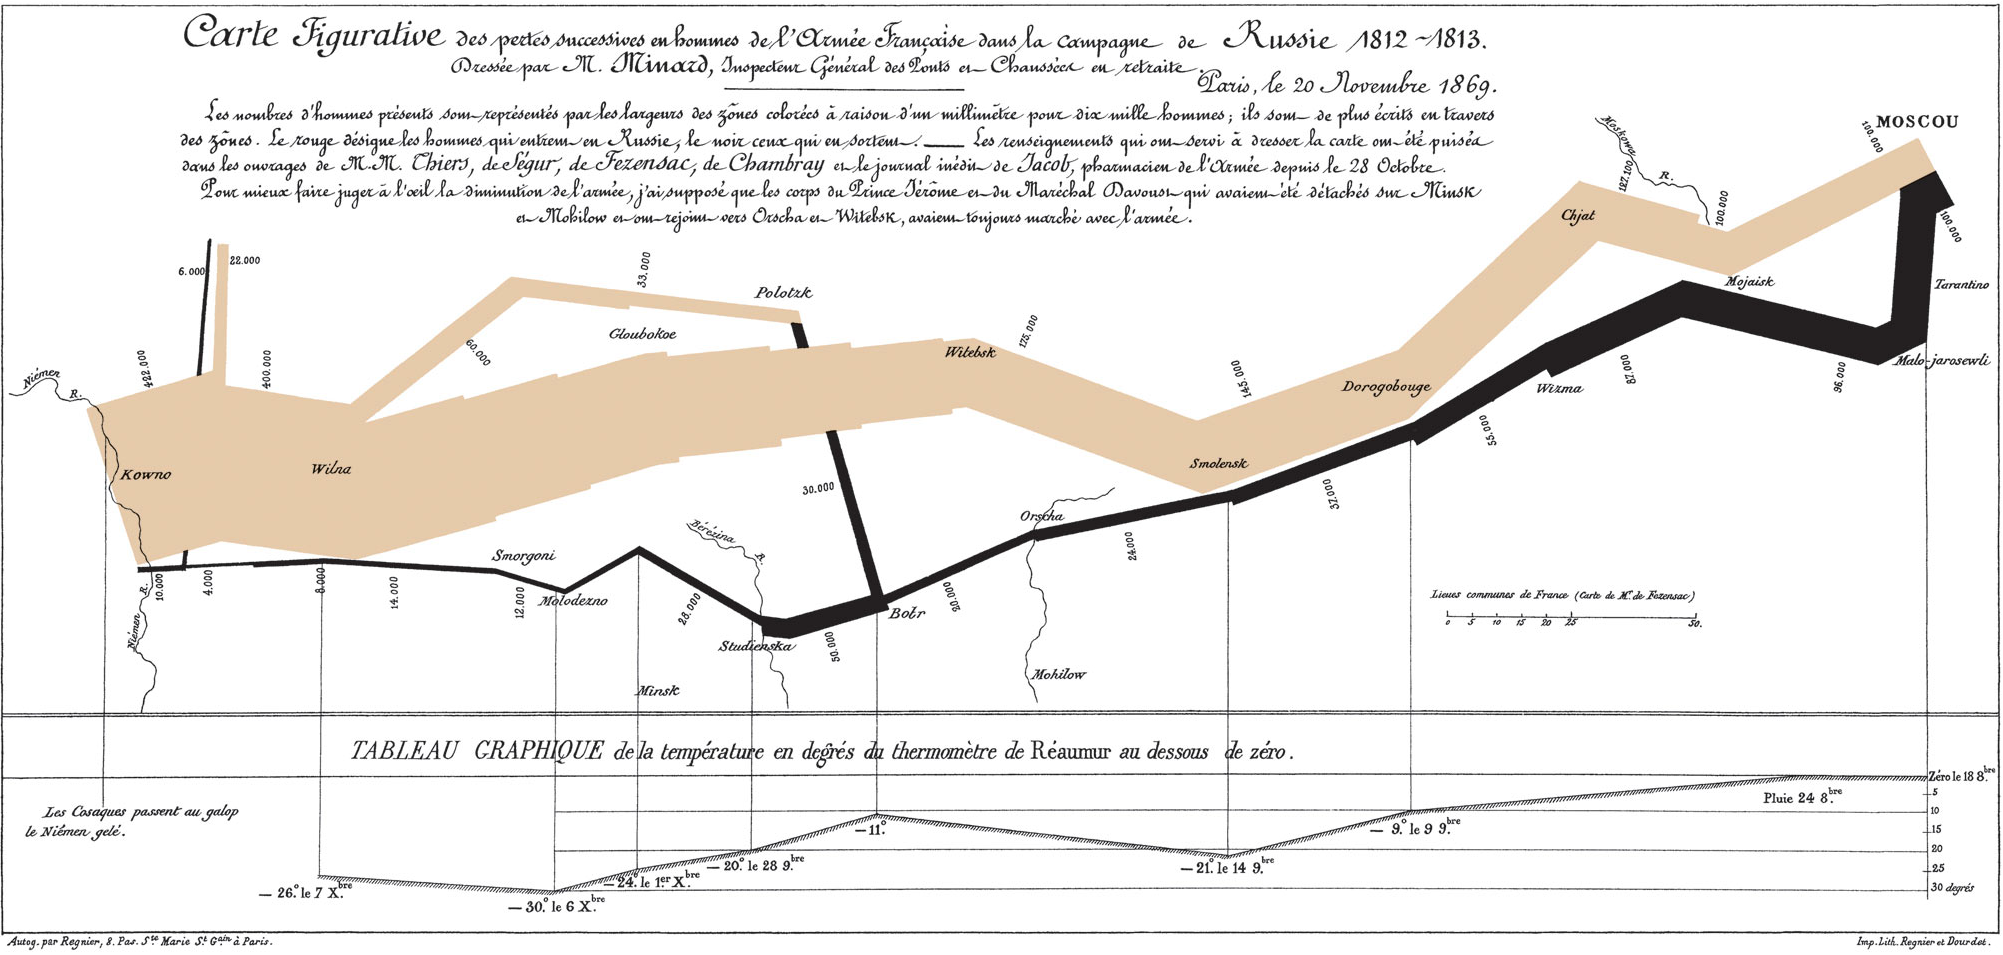
\includegraphics[width=.90\textwidth]{pictures/Minard.png}
    \caption{by Charles Joseph Minard, 1869}
\end{figure}
\end{frame}

\begin{frame}[fragile]{Afgrænsning}
\protect\hypertarget{afgruxe6nsning}{}
Jeg (regner med) at snakke \textbf{en del} om:

\begin{itemize}
\item
  Hvorfor vi gider arbejde med \textbf{spatiale} datakilder
\item
  Hvordan vi arbejder med spatiale datakilder
\item
  Hvordan vi kan bruge spatiale datakilder til at \textbf{visualisere}
  andre dimensioner i data
\item
  Hvordan vi gør det i \texttt{R}
\end{itemize}

\bigskip

Jeg kommer \textbf{ikke} til at snakke (så meget) om:

\begin{itemize}
\item
  Datawrangling og -manipulation med geospatial data
\item
  Datavisualisering generelt
\end{itemize}
\end{frame}

\begin{frame}{Eksempler på spatiale datavisualiseringer}
\protect\hypertarget{eksempler-puxe5-spatiale-datavisualiseringer}{}
\columnsbegin

\column{.5\textwidth}

\onslide <2->
\begin{figure}[H]
    \centering
    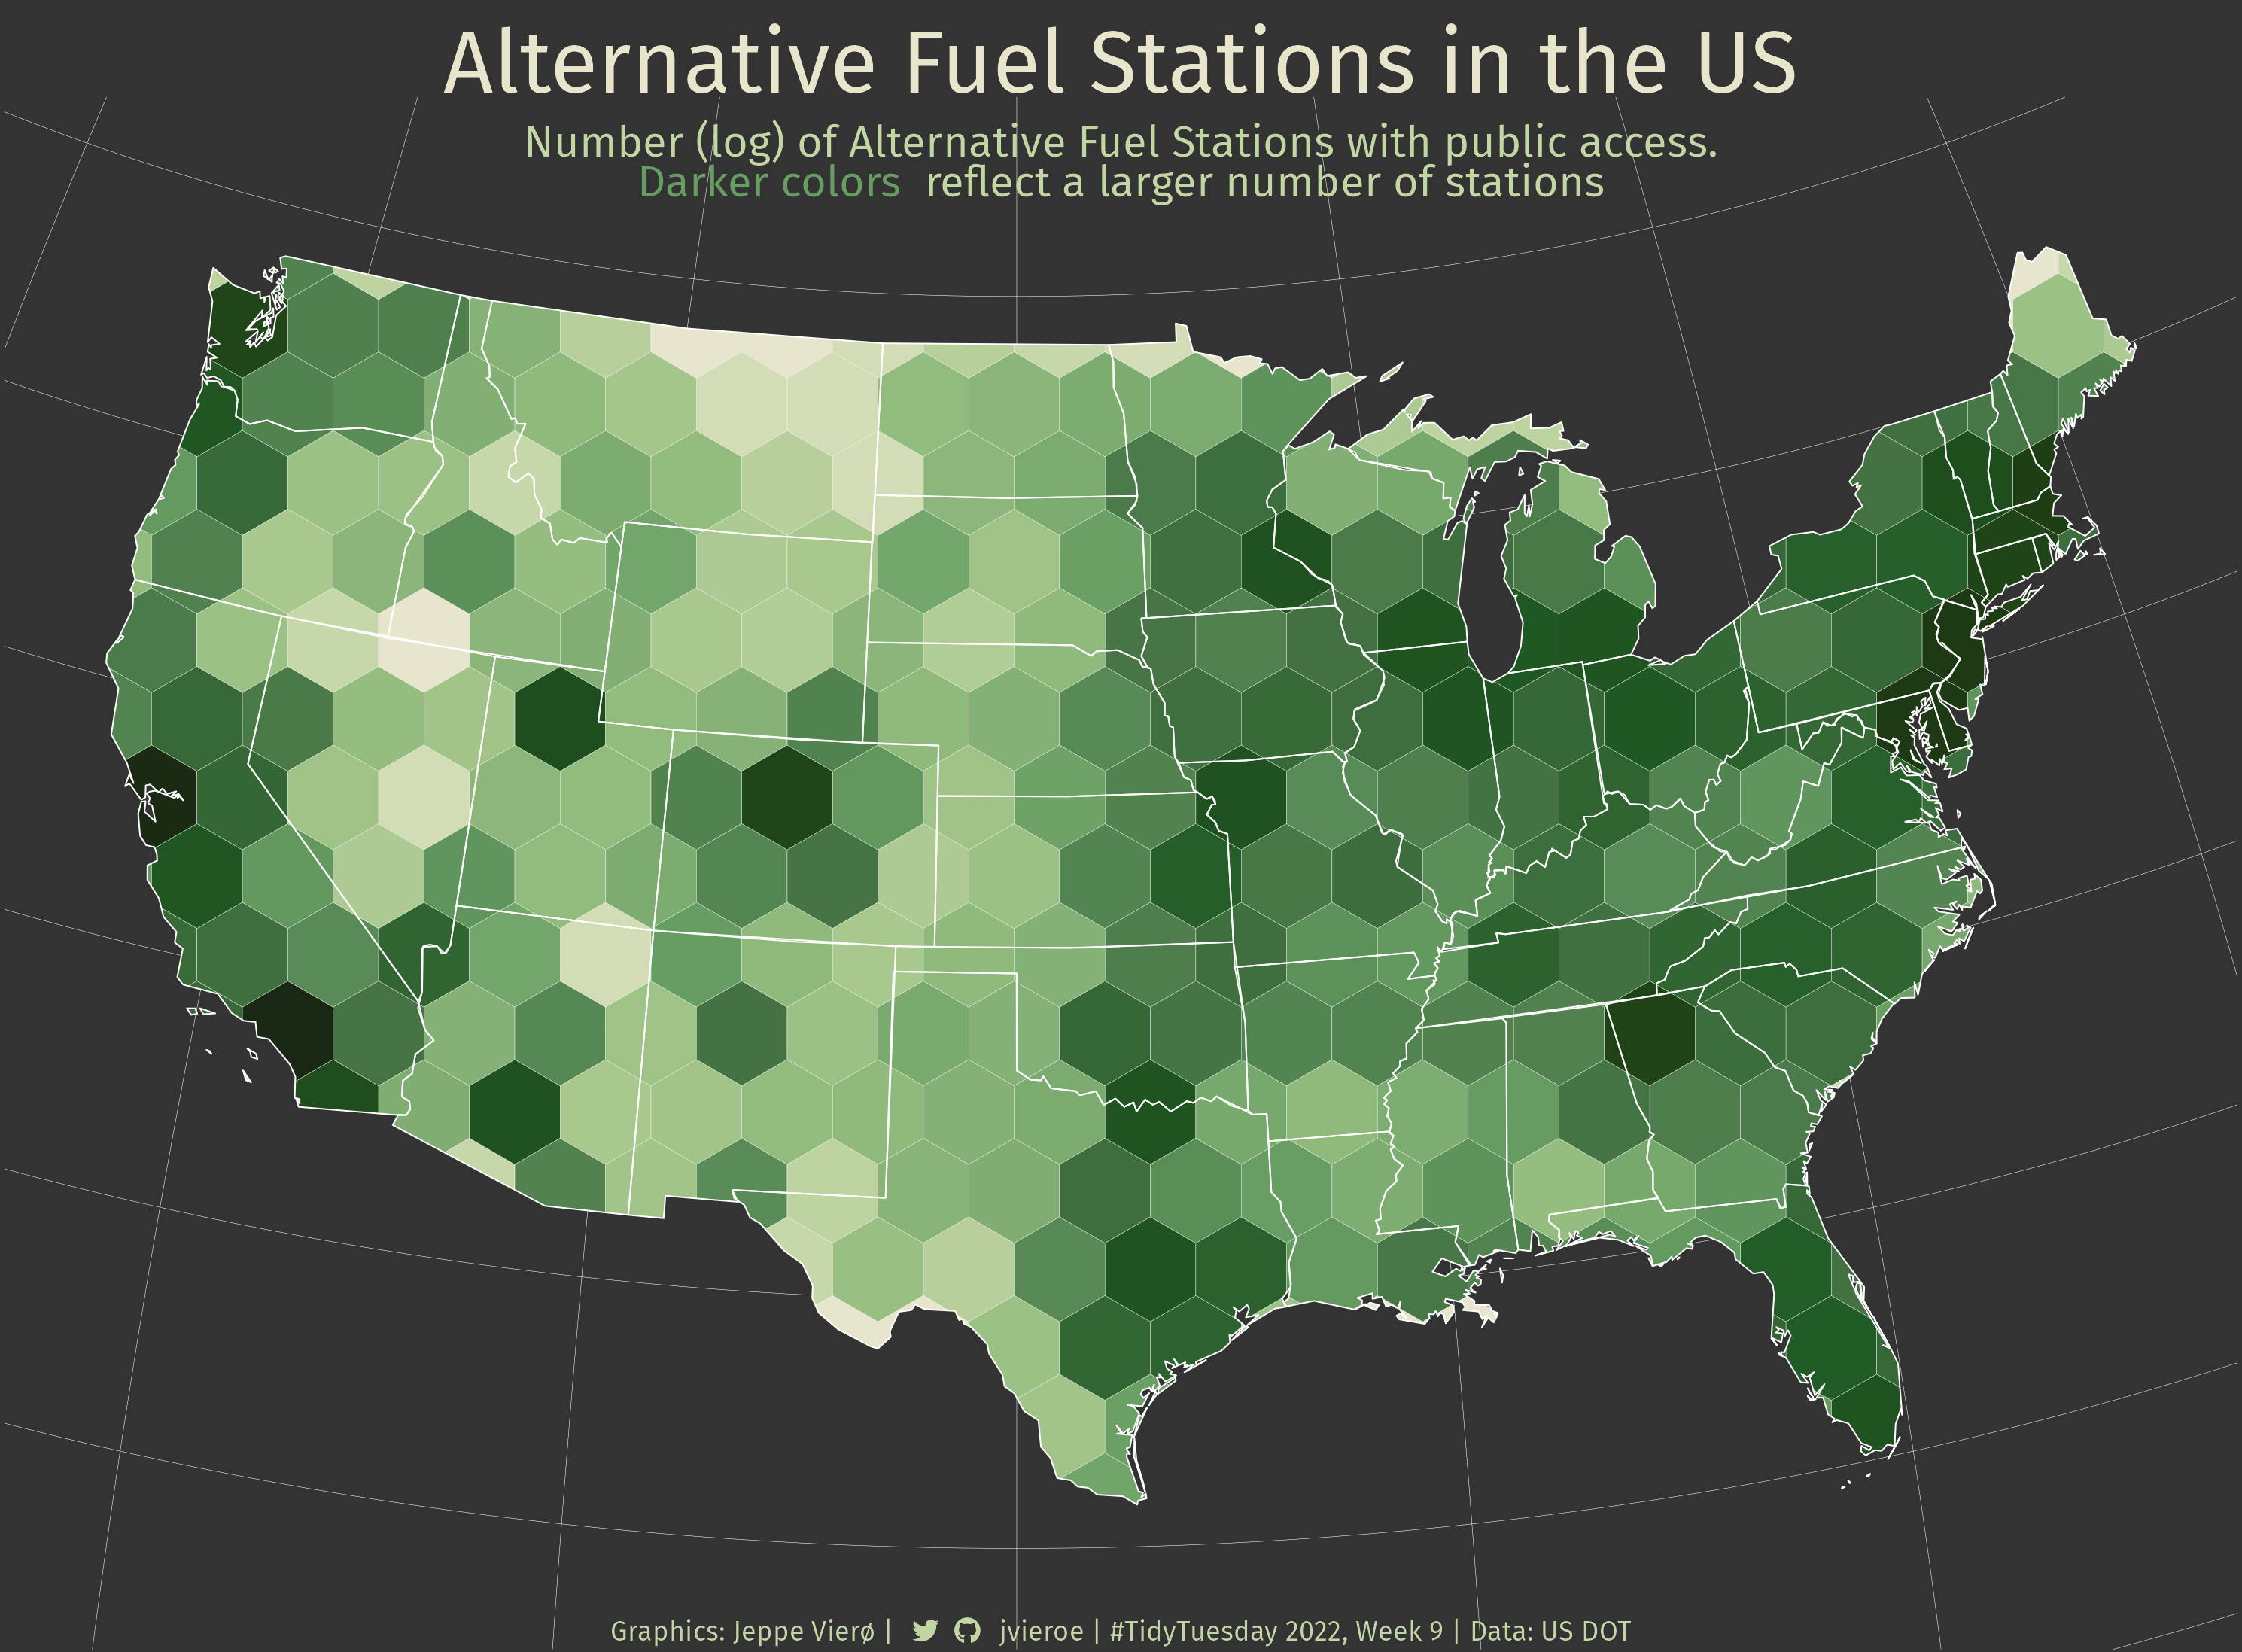
\includegraphics[width=.90\textwidth]{pictures/fuel.png}
\end{figure}

\column{.5\textwidth}

\onslide <3->
\begin{figure}[H]
    \centering
    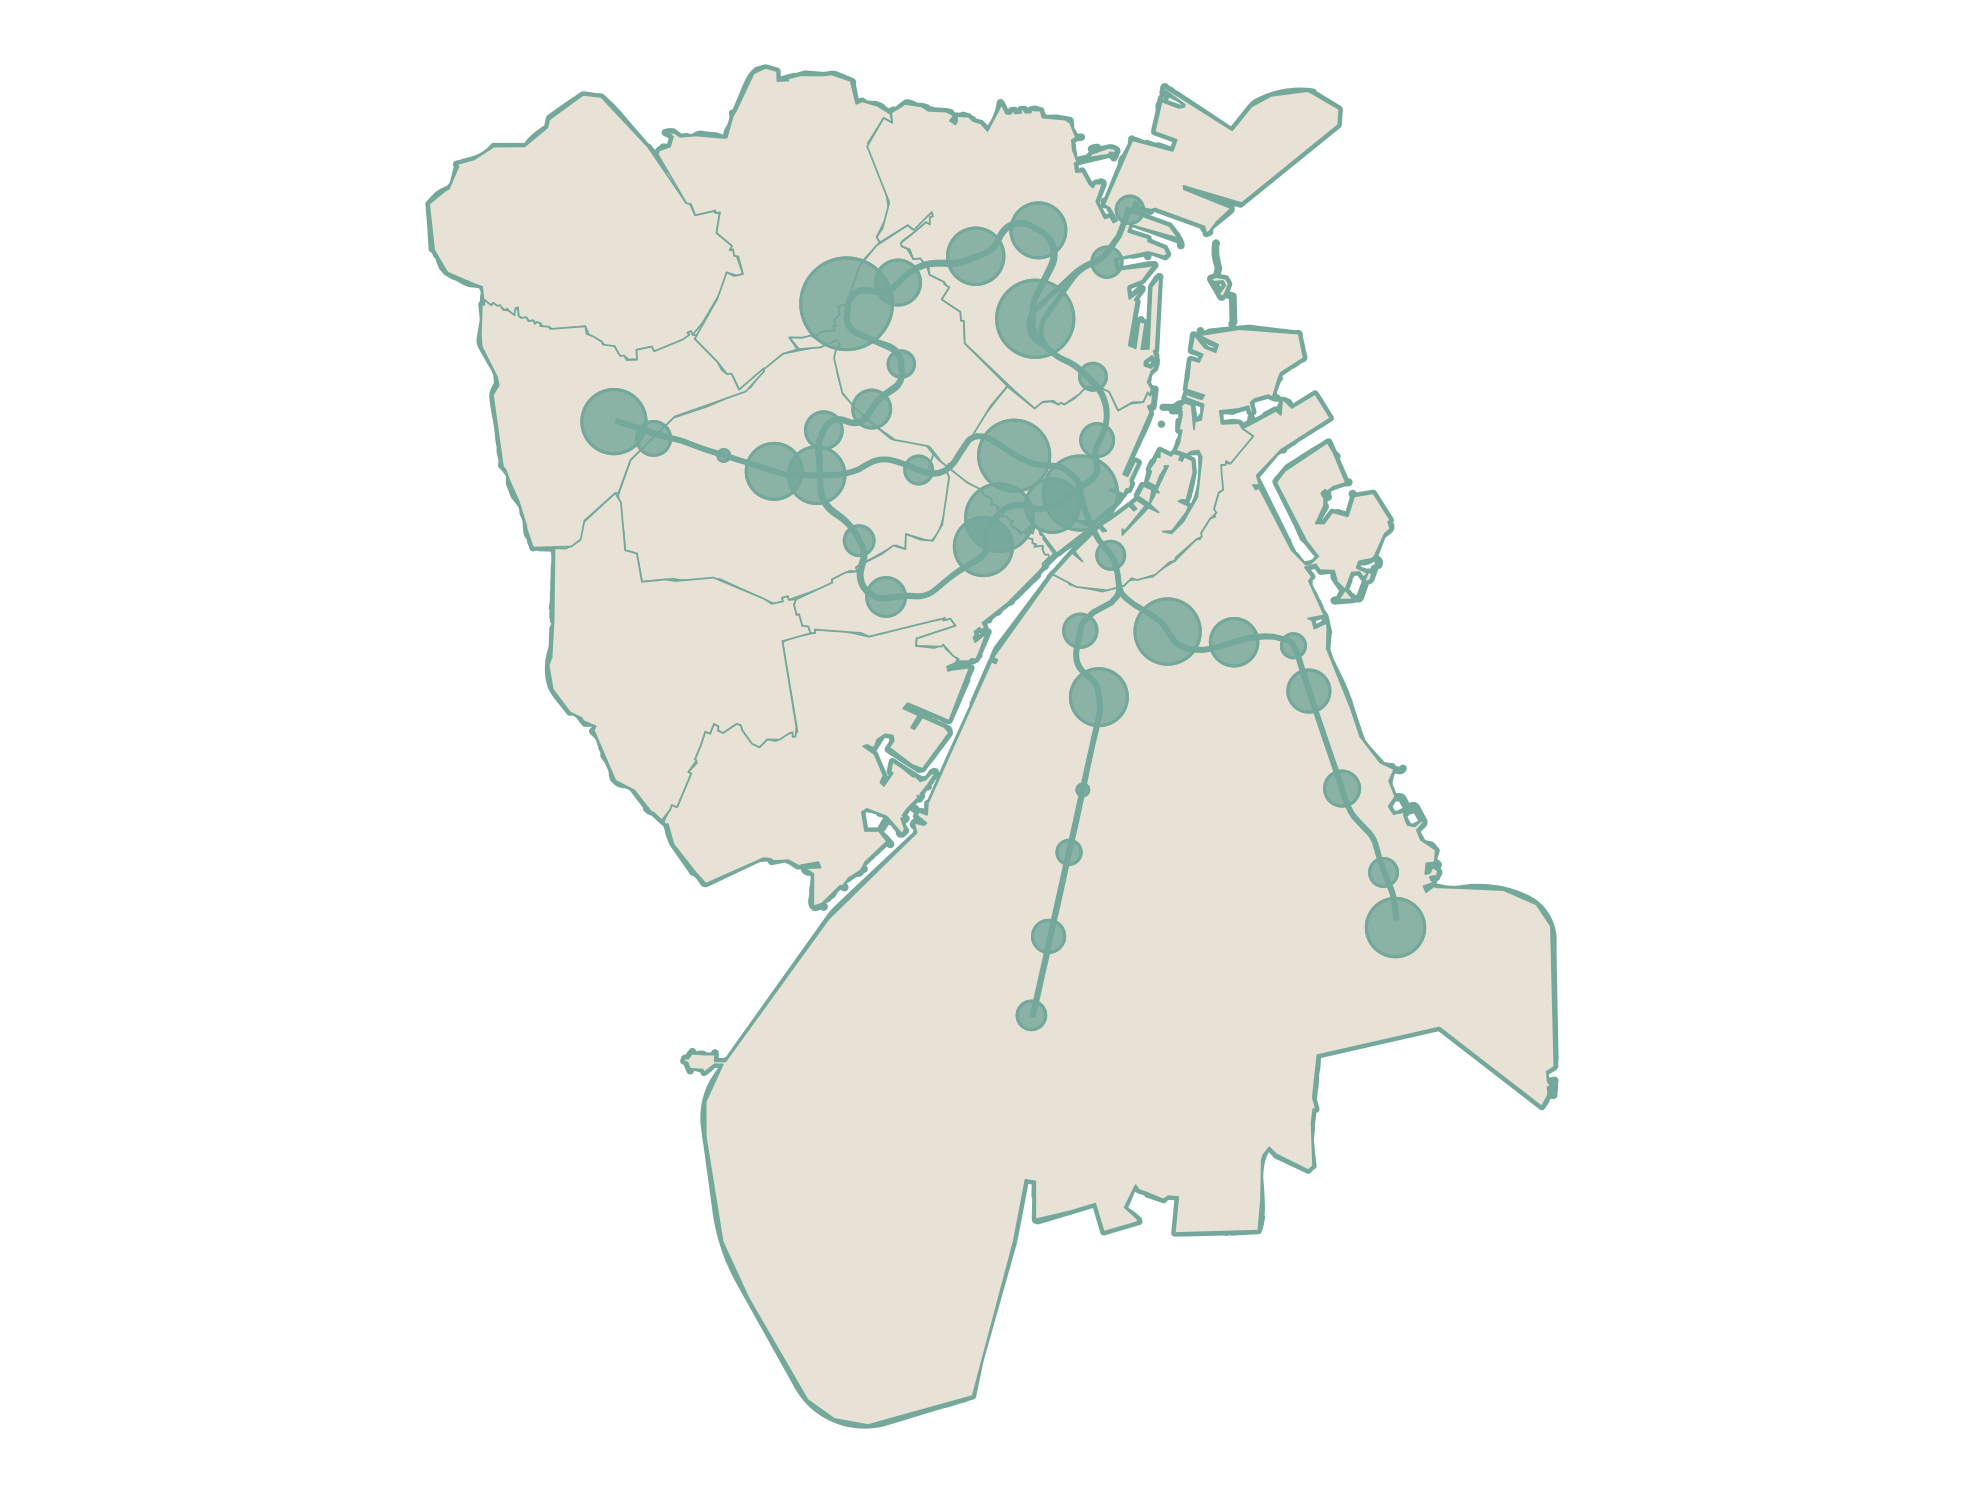
\includegraphics[width=.90\textwidth]{pictures/Forstadsbilister_start.png}
\end{figure}

\columnsend
\end{frame}

\begin{frame}{Eksempler på spatiale datavisualiseringer}
\protect\hypertarget{eksempler-puxe5-spatiale-datavisualiseringer-1}{}
\columnsbegin

\column{.4\textwidth}

\onslide <1->
\begin{figure}[H]
    \centering
    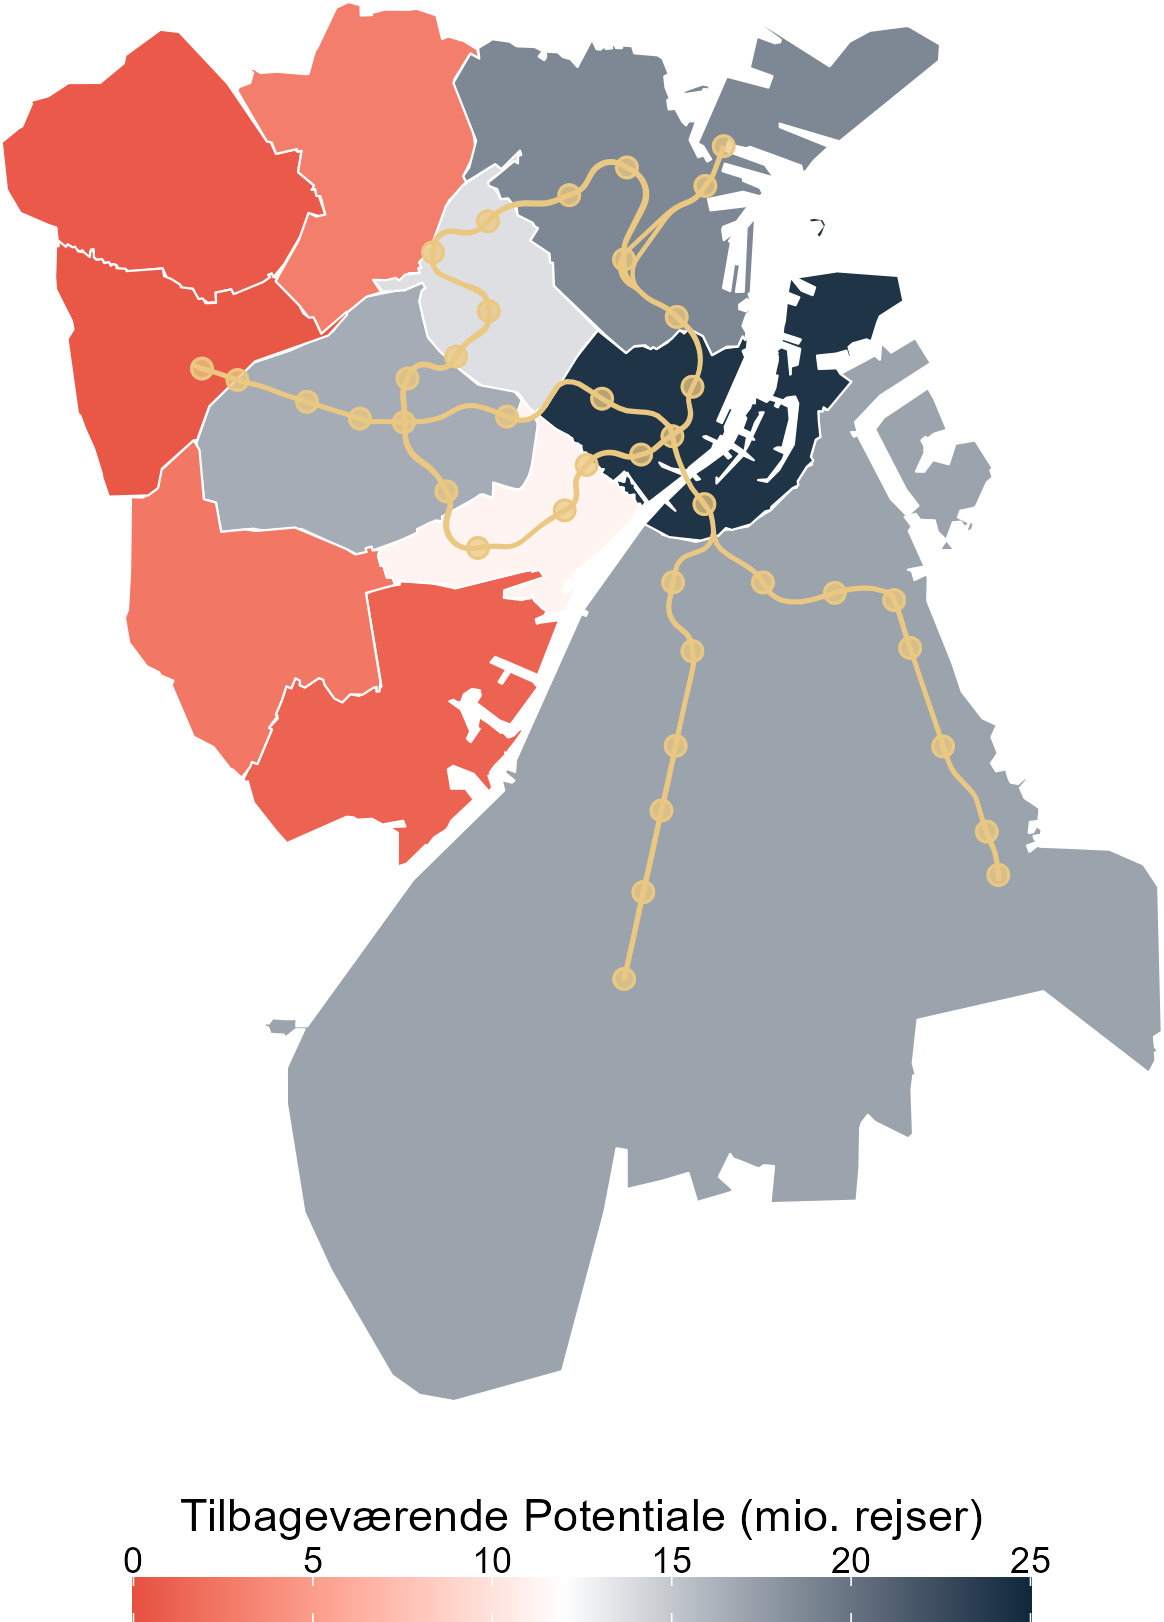
\includegraphics[width=.70\textwidth]{pictures/potentialeudnyttelse_absolut.png}
\end{figure}

\column{.6\textwidth}

\onslide <2->
\begin{figure}[H]
    \centering
    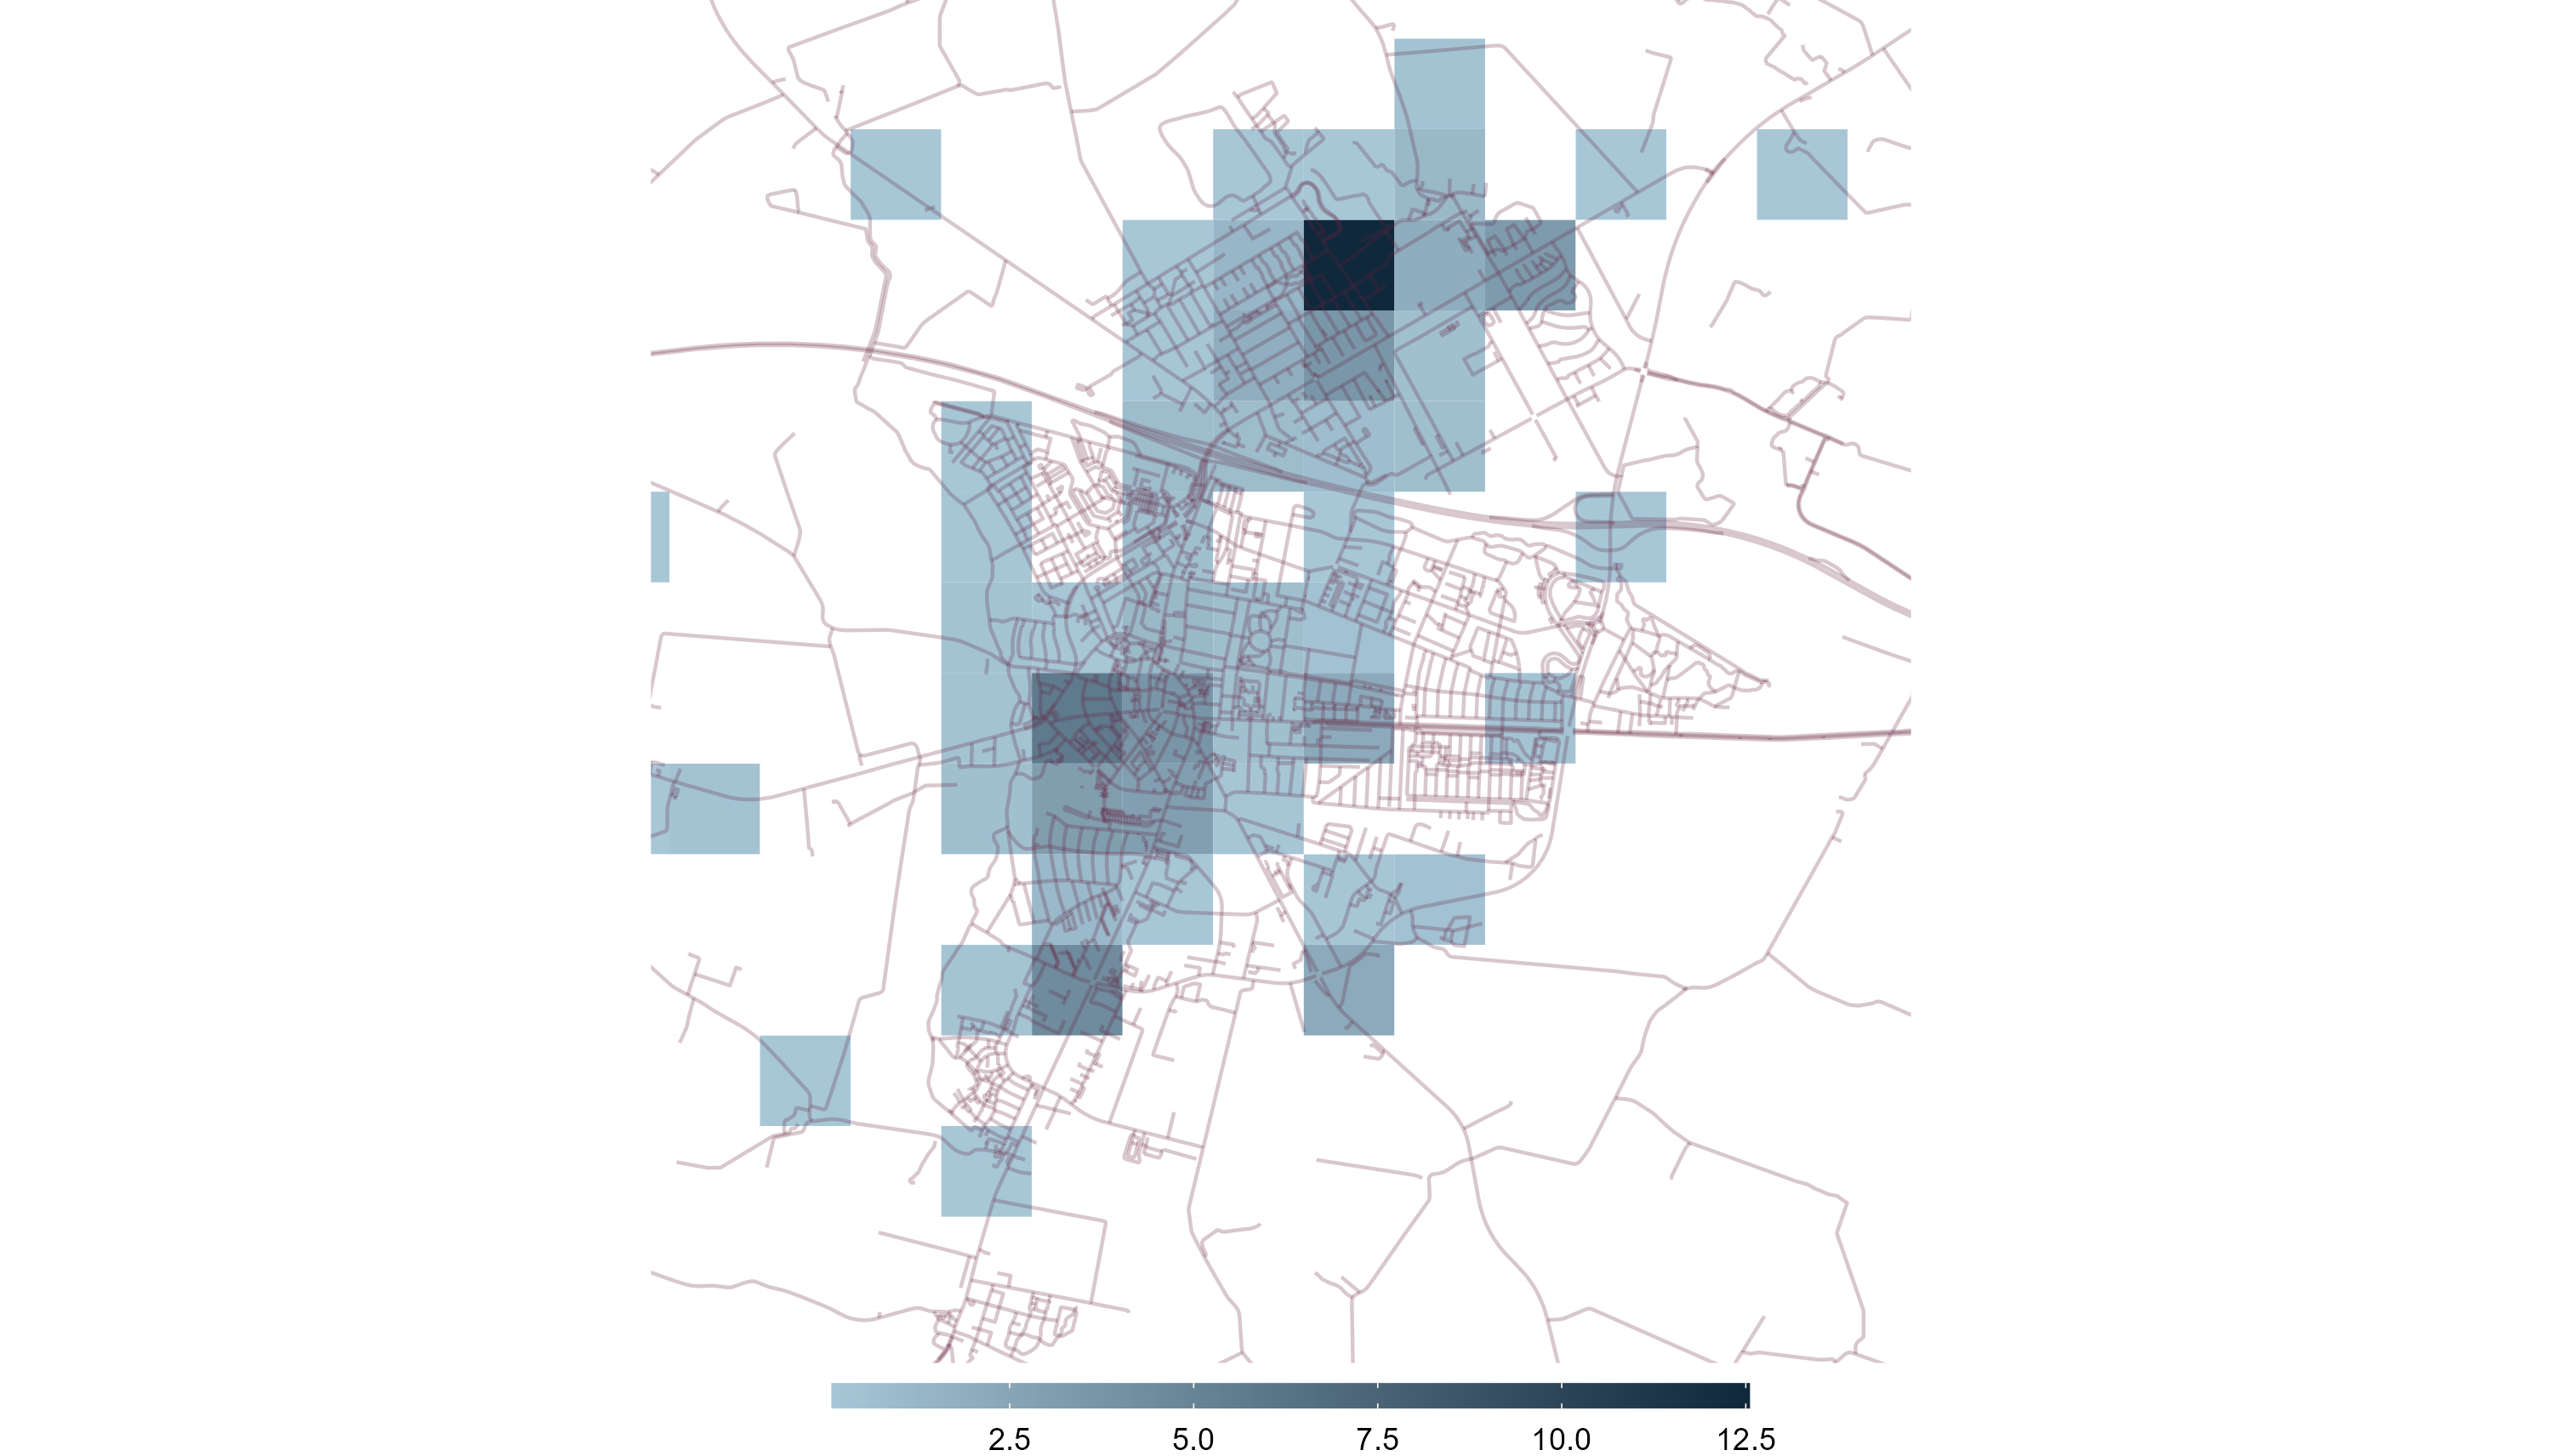
\includegraphics[width=.99\textwidth]{pictures/hex_ringsted.png}
\end{figure}

\columnsend
\end{frame}

\begin{frame}{Hvorfor skal vi arbejde med spatialt data?}
\protect\hypertarget{hvorfor-skal-vi-arbejde-med-spatialt-data}{}
\tiny

\normalsize

\columnsbegin
\column{.5\textwidth}

\tiny

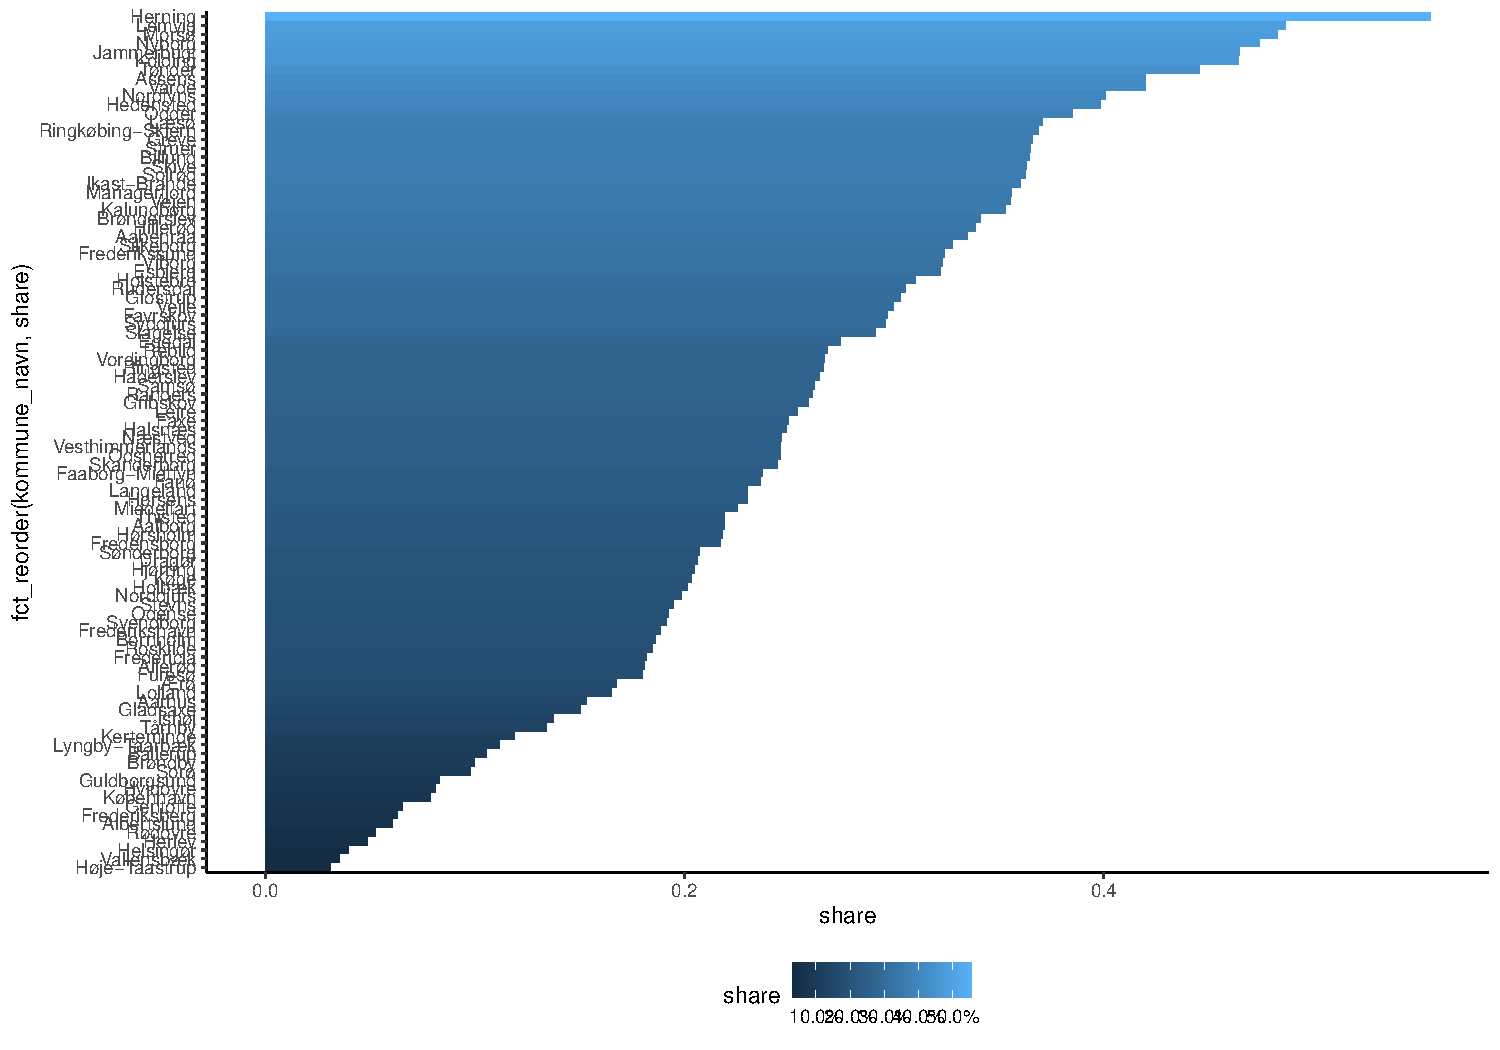
\includegraphics[width=1\linewidth]{crashcourse_slides_files/figure-beamer/unnamed-chunk-2-1}

\normalsize

\column{.5\textwidth}

\tiny

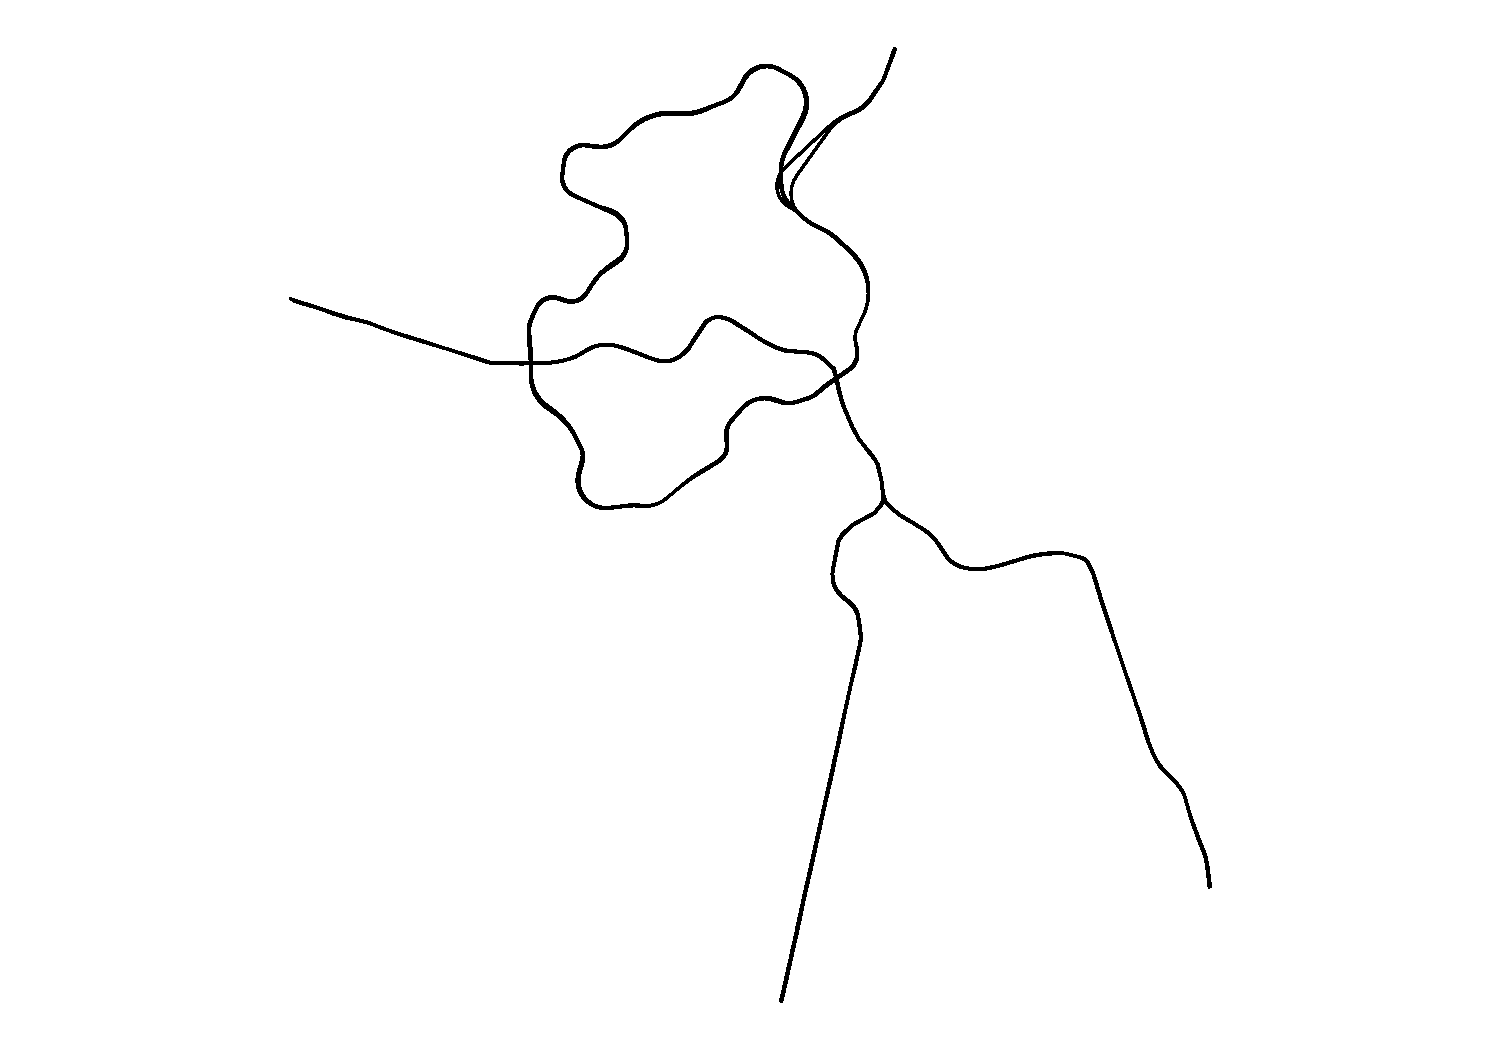
\includegraphics[width=1\linewidth]{crashcourse_slides_files/figure-beamer/unnamed-chunk-3-1}

\normalsize

\columnsend
\end{frame}

\begin{frame}{Hvorfor skal vi arbejde med spatialt data?}
\protect\hypertarget{hvorfor-skal-vi-arbejde-med-spatialt-data-1}{}
\columnsbegin

\column{.5\textwidth}

Typisk kan man med fordel (overveje at) visualisere sit data grafisk,
hvis

\begin{itemize}
\tightlist
\item
  Der er nogle \textbf{substantielle geografiske mønstre} i data, der er
  interessante (case in point:)
\end{itemize}

og/eller,

\begin{itemize}
\tightlist
\item
  Det data, vi gerne vil visualisere fundamentalt set har en tydelig
  geografisk dimension, selvom der ikke er noget geografisk mønster. Her
  vil en geografisk fremstilling ikke bidrage substantielt men hjælpe
  modtageren med en klar reference
\end{itemize}

\column{.5\textwidth}

\tiny

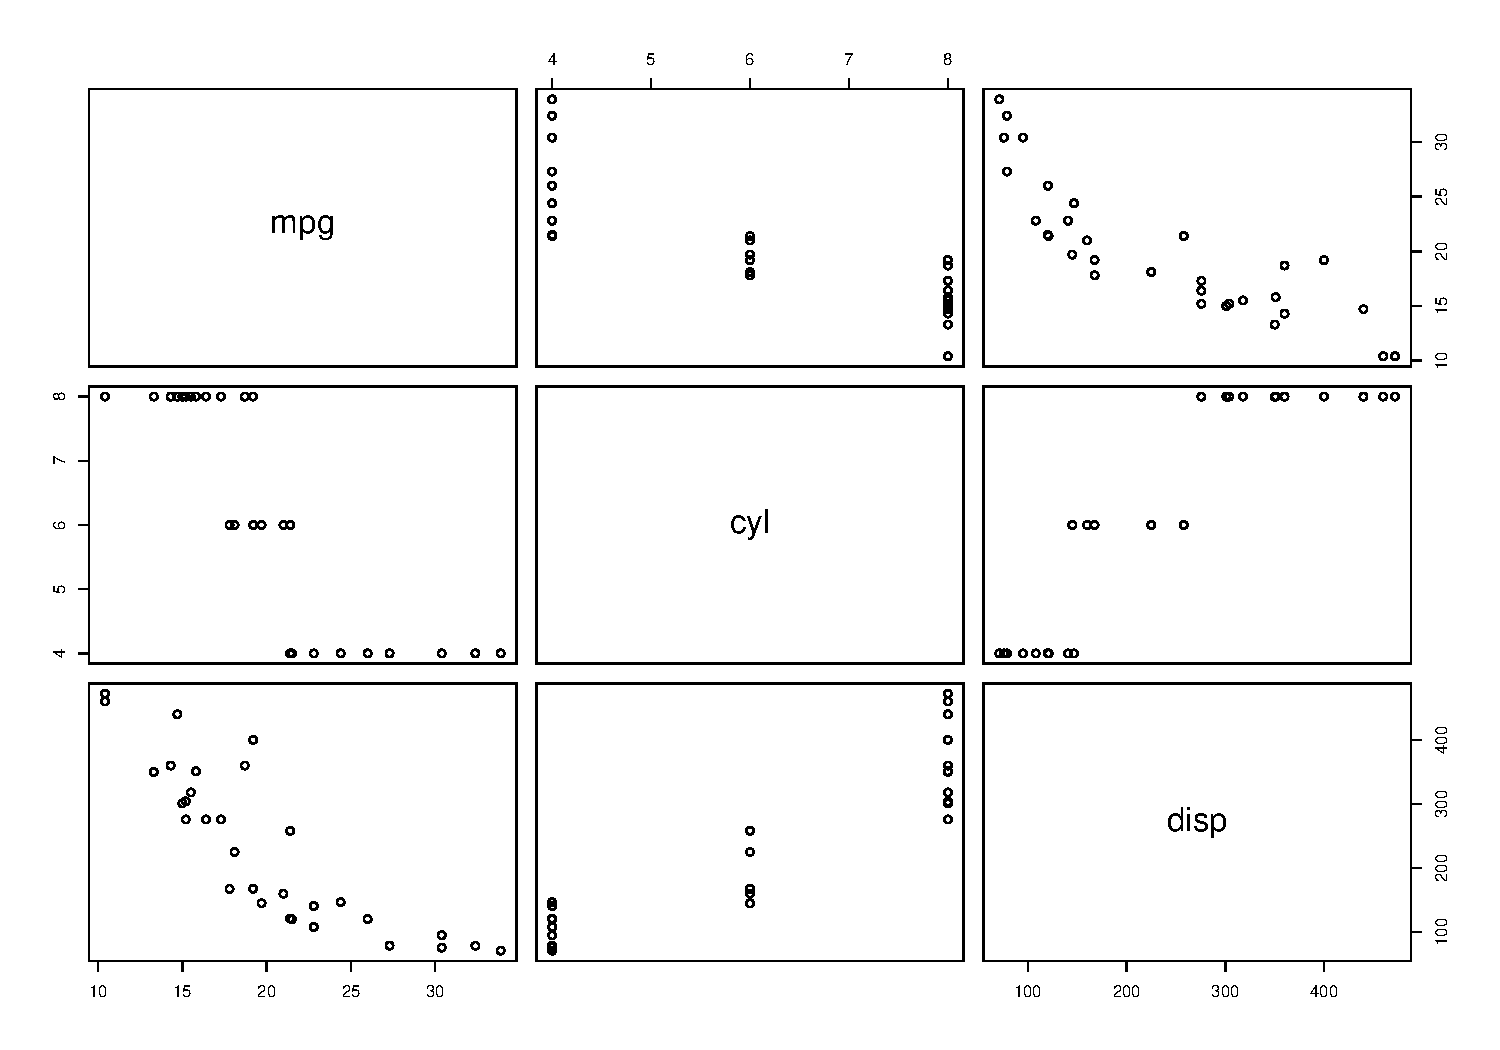
\includegraphics[width=1\linewidth]{crashcourse_slides_files/figure-beamer/unnamed-chunk-4-1}

\normalsize

\columnsend
\end{frame}

\begin{frame}{Hvorfor skal vi arbejde med spatialt data?}
\protect\hypertarget{hvorfor-skal-vi-arbejde-med-spatialt-data-2}{}
\begin{itemize}
\item
  Kort er fede, fordi de er de \textbf{eneste visualiseringer, hvor alle
  har en intuitiv og umiddelbar forståelse af X- og Y-aksen}
\item
  Det er smart, fordi det frigør lidt (kognitiv) plads til at
  visualisere flere andre \emph{dimensioner} i data ved hjælp af farve,
  størrelse osv. (`aesthetics')
\item
  Tit arbejder vi (også i Epinion) med geografiske enheder uden at tænke
  nærmere over det:

  \begin{itemize}
  \tightlist
  \item
    danske skoler,
  \item
    valgkredse til FT-valg,
  \item
    metrostationer i København,
  \item
    norske jerbaneruter osv.
  \end{itemize}
\item
  Her kan det (måske) give mening at visualisere nogle af sine pointer
  ved hjælp af geografiske datavisualiseringer
\item
  \ldots{} hvilket er en lang måde at sige ``kort'' på
\end{itemize}
\end{frame}

\hypertarget{the-basics-geodata-spatialt-data}{%
\section{The Basics: Geodata / spatialt
data}\label{the-basics-geodata-spatialt-data}}

\begin{frame}{Hvad er (geo)spatialt data?}
\protect\hypertarget{hvad-er-geospatialt-data}{}
\begin{itemize}
\item
  ``Spatial data'' er basically alt data, hvor observationer har en form
  for placering/relation ift. hinanden
\item
  Typisk bliver det brugt i den lidt mere snævre forstand (=
  \textbf{geospatial} data), hvor fokus er på geografiske
  placeringer/relationer
\item
  Klassiske eksempler på spatialt data er digitaliserede kort over
  landegrænser, landbrugsafkast, vejnetværk, togstationer osv.
\item
  Her består den spatiale dimension af det geografiske element:
  \emph{hvad} ligger \emph{hvor}
\end{itemize}
\end{frame}

\begin{frame}{Datastrukturer og typer af geodata}
\protect\hypertarget{datastrukturer-og-typer-af-geodata}{}
Grundlæggende arbejder vi med \textbf{tre typer af geospatiale
datakilder}

Hver type har en (nogenlunde) parallel til graftyper, I er vant til at
arbejde med:

\bigskip

\begin{enumerate}
\tightlist
\item
  \textbf{Punkter}
\end{enumerate}

\begin{itemize}
\tightlist
\item
  Tænk på dem som almindelige \emph{punkter i et scatterplot}
\end{itemize}

\begin{enumerate}
\setcounter{enumi}{1}
\tightlist
\item
  \textbf{Linjer}
\end{enumerate}

\begin{itemize}
\tightlist
\item
  Tænk på dem som \emph{linjer i et linechart}
\end{itemize}

\begin{enumerate}
\setcounter{enumi}{2}
\tightlist
\item
  \textbf{Polygoner}
\end{enumerate}

\begin{itemize}
\tightlist
\item
  Her er parallelen ikke lige så tydelig
\item
  \ldots{} men i en data viz-kontekst kan I tænke på dem som
  \emph{søjler i et bar chart} (ish\ldots)
\end{itemize}
\end{frame}

\begin{frame}{(1) Punkter}
\protect\hypertarget{punkter}{}
\columnsbegin
\column{.4\textwidth}

\begin{itemize}
\item
  Punkter består af simple koordinater (x, y), der refererer til en
  specifik lokation
\item
  Punkter har ingen størrelse (og intet \emph{areal}), de er uendeligt
  små
\item
  Eksempler: byer, stationer, skoler osv.
\end{itemize}

\column{.6\textwidth}

\tiny

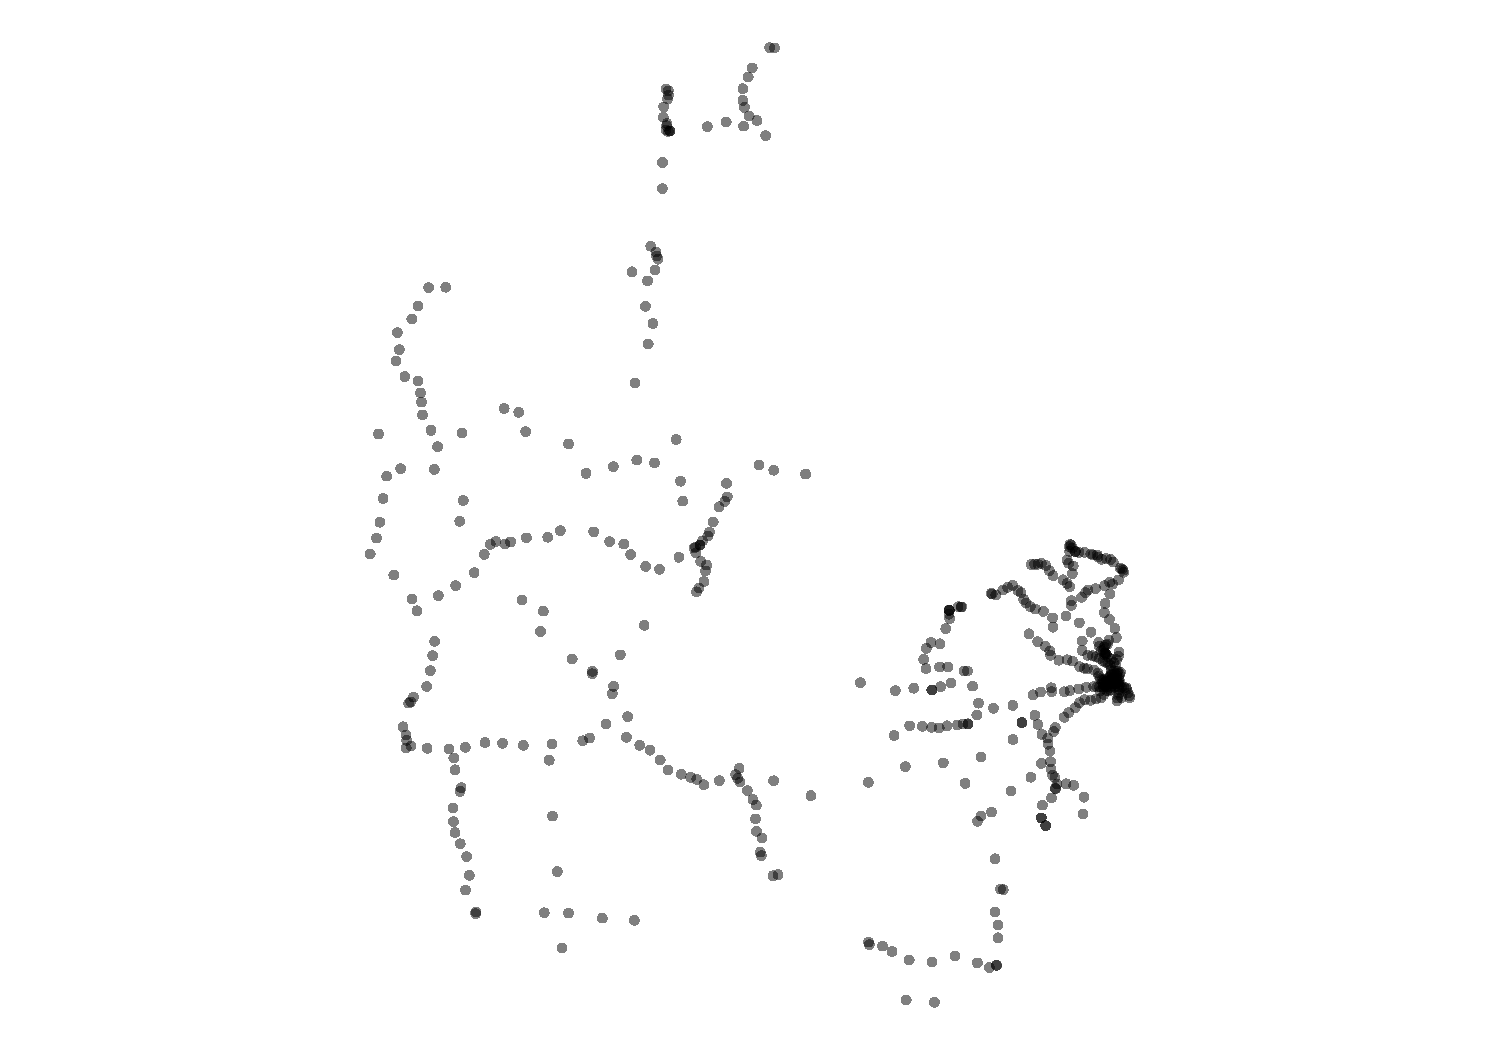
\includegraphics[width=1\linewidth]{crashcourse_slides_files/figure-beamer/unnamed-chunk-5-1}

\normalsize

\columnsend
\end{frame}

\begin{frame}{(2) Linjer}
\protect\hypertarget{linjer}{}
\columnsbegin
\column{.4\textwidth}

\begin{itemize}
\item
  Linjer består -- grundlæggende -- af punkter, der er kombineret til en
  \emph{linestring} vha. en defineret rækkefølge
\item
  Konstruktionen er sjældent noget, I skal bekymre jer om: linjedata
  ligger typisk opbevaret som linjer (\(\neq\) punkter). Her er det bare
  plug 'n play
\item
  Linjer har intet \emph{areal} (fordi de består af punkter)
\item
  Eksempler: veje, floder, jernbanenetværk osv.
\end{itemize}

\column{.6\textwidth}

\tiny

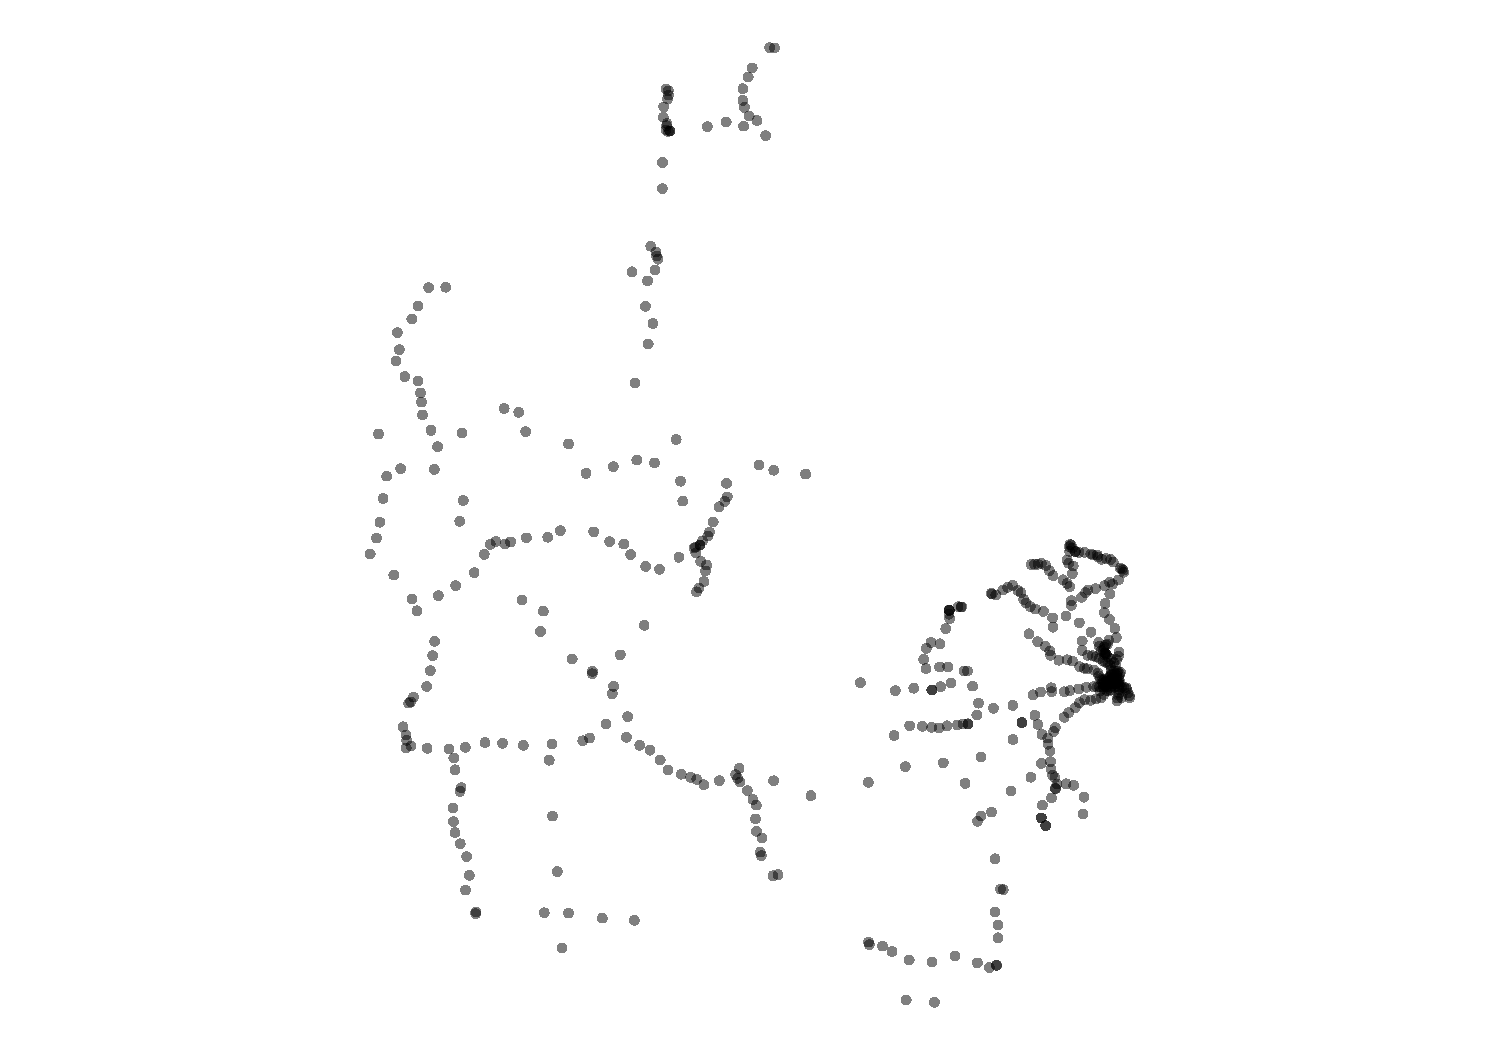
\includegraphics[width=1\linewidth]{crashcourse_slides_files/figure-beamer/unnamed-chunk-6-1}

\normalsize

\columnsend
\end{frame}

\begin{frame}{(3) Polygoner}
\protect\hypertarget{polygoner}{}
\columnsbegin
\column{.4\textwidth}

\begin{itemize}
\item
  Polygoner består -- ligesom linjer -- af punkter, der er kombineret
  til en \emph{polygon} vha. en defineret rækkefølge. Igen, det er
  sjældent noget, I skal bekymre jer om
\item
  Forskellen er, at polygoner er \emph{lukkede linjer}, der former et
  afgrænset område
\item
  De kan have alle tænkelige former. Det centrale er, at polygoner har
  et \emph{areal}
\item
  Eksempler: stater, kommuner, valgkredse osv.
\end{itemize}

\column{.6\textwidth}

\tiny

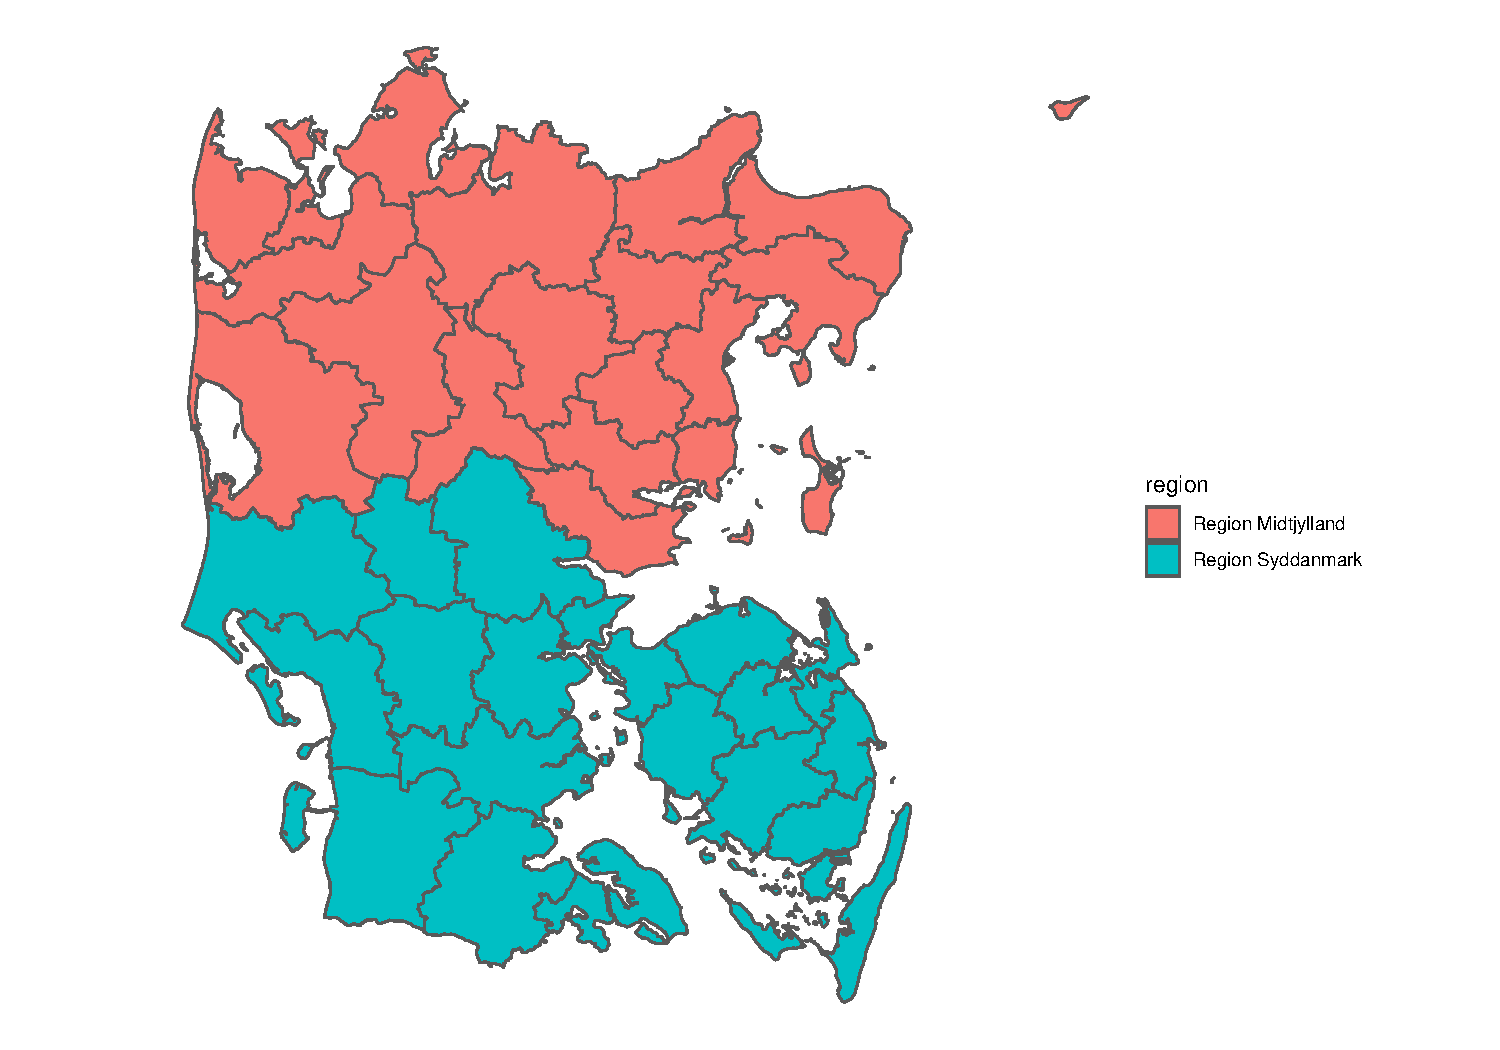
\includegraphics[width=1\linewidth]{crashcourse_slides_files/figure-beamer/unnamed-chunk-7-1}

\normalsize

\columnsend
\end{frame}

\hypertarget{the-basics-spatialt-data-i-r}{%
\section{\texorpdfstring{The Basics: Spatialt data i
\texttt{R}}{The Basics: Spatialt data i R}}\label{the-basics-spatialt-data-i-r}}

\begin{frame}[fragile]{Hvordan arbejder vi med spatialt data?}
\protect\hypertarget{hvordan-arbejder-vi-med-spatialt-data}{}
\begin{itemize}
\item
  Den typiske måde at lege med spatialt data på er vha. GIS (Geographic
  Information Systems)-værktøjer designet til det

  \begin{itemize}
  \tightlist
  \item
    QGis, ArcGIS osv.
  \end{itemize}
\item
  Programmer som \texttt{R} er dog løbende blevet udvidet med pakker,
  der gør det muligt at klare alting i det samme stykke software, som
  man bruger til andre ting
\item
  Det er dobbelt smart, fordi man har alting ét sted og bygget op
  omkring kode, der kan ændres og opdateres
\item
  Med \texttt{sf} er det blevet
  \href{https://www.nickbearman.me.uk/2019/04/spatial-r-moving-from-sp-to-sf/}{smooth
  sailing}. Den måde, pakken håndterer det \emph{spatiale} aspekt af et
  datasæt gør, at det ligner alle andre datasæt til forveksling
\end{itemize}
\end{frame}

\begin{frame}[fragile]{A Blast from the Past: \{\texttt{sp}\}}
\protect\hypertarget{a-blast-from-the-past-sp}{}
\tiny

\normalsize

\begin{itemize}
\item
  Det har tidligere været relativt besværligt at arbejde med spatialt
  data i \texttt{R}
\item
  \texttt{sp}-pakken var det førende framework, men selv simple datasæt
  var\ldots{} irriterende:
\end{itemize}

\begin{figure}[H]
    \centering
    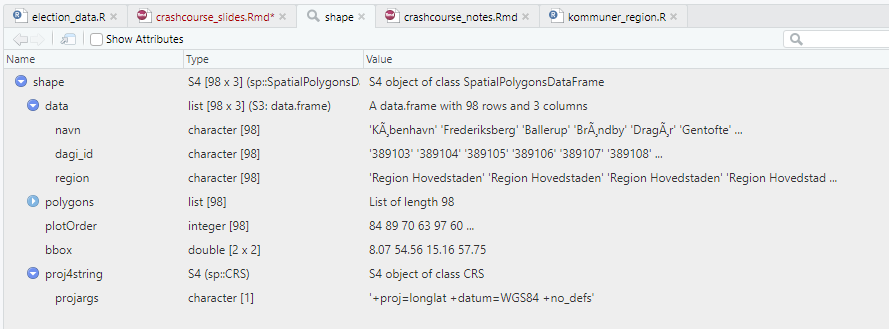
\includegraphics[width=.90\textwidth]{pictures/sp.png}
\end{figure}
\end{frame}

\begin{frame}[fragile]{Din nye bedste ven: \{\texttt{sf}\}}
\protect\hypertarget{din-nye-bedste-ven-sf}{}
\begin{itemize}
\item
  Lad os kigge på det!
\item
  Til at starte med loader vi et datasæt over danske kommuner:
\end{itemize}

\tiny

\begin{Shaded}
\begin{Highlighting}[]
\FunctionTok{library}\NormalTok{(tidyverse)}
\FunctionTok{library}\NormalTok{(sf)}

\NormalTok{df }\OtherTok{\textless{}{-}} \FunctionTok{st\_read}\NormalTok{(}\AttributeTok{dsn =} \StringTok{"data/kommuner"}\NormalTok{,}
              \AttributeTok{layer =} \StringTok{"kommuner"}\NormalTok{)}
\end{Highlighting}
\end{Shaded}

\normalsize

\tiny

\begin{Shaded}
\begin{Highlighting}[]
\NormalTok{df}
\end{Highlighting}
\end{Shaded}

\begin{verbatim}
## Simple feature collection with 98 features and 3 fields
## Geometry type: MULTIPOLYGON
## Dimension:     XY
## Bounding box:  xmin: 8.07251 ymin: 54.55908 xmax: 15.15738 ymax: 57.75257
## Geodetic CRS:  WGS 84
## First 10 features:
##             navn dagi_id             region                       geometry
## 1      København  389103 Region Hovedstaden MULTIPOLYGON (((12.54502 55...
## 2  Frederiksberg  389104 Region Hovedstaden MULTIPOLYGON (((12.53735 55...
## 3       Ballerup  389105 Region Hovedstaden MULTIPOLYGON (((12.3423 55....
## 4        Brøndby  389106 Region Hovedstaden MULTIPOLYGON (((12.44279 55...
## 5         Dragør  389107 Region Hovedstaden MULTIPOLYGON (((12.64513 55...
## 6       Gentofte  389108 Region Hovedstaden MULTIPOLYGON (((12.59175 55...
## 7       Gladsaxe  389109 Region Hovedstaden MULTIPOLYGON (((12.47771 55...
## 8       Glostrup  389110 Region Hovedstaden MULTIPOLYGON (((12.41842 55...
## 9         Herlev  389111 Region Hovedstaden MULTIPOLYGON (((12.40838 55...
## 10   Albertslund  389112 Region Hovedstaden MULTIPOLYGON (((12.36431 55...
\end{verbatim}

\normalsize
\end{frame}

\begin{frame}[fragile]{Din nye bedste ven: \{\texttt{sf}\}}
\protect\hypertarget{din-nye-bedste-ven-sf-1}{}
\begin{itemize}
\tightlist
\item
  Magien ligger i \texttt{geometry}-listen. Alt (!) andet er data
  frames/tibbles, som I kender dem
\end{itemize}

\tiny

\begin{Shaded}
\begin{Highlighting}[]
\FunctionTok{glimpse}\NormalTok{(df)}
\end{Highlighting}
\end{Shaded}

\begin{verbatim}
## Rows: 98
## Columns: 4
## $ navn     <chr> "København", "Frederiksberg", "Ballerup", "Brøndby", "Dragør"~
## $ dagi_id  <chr> "389103", "389104", "389105", "389106", "389107", "389108", "~
## $ region   <chr> "Region Hovedstaden", "Region Hovedstaden", "Region Hovedstad~
## $ geometry <MULTIPOLYGON [°]> MULTIPOLYGON (((12.54502 55..., MULTIPOLYGON (((~
\end{verbatim}

\normalsize

\begin{itemize}
\tightlist
\item
  Derfor kan vi også med et snuptag konvertere det hele om til at rent
  og ikke-spatialt datasæt:
\end{itemize}

\tiny

\begin{Shaded}
\begin{Highlighting}[]
\NormalTok{df }\SpecialCharTok{\%\textgreater{}\%} 
  \FunctionTok{st\_drop\_geometry}\NormalTok{() }\SpecialCharTok{\%\textgreater{}\%} 
  \FunctionTok{glimpse}\NormalTok{(.)}
\end{Highlighting}
\end{Shaded}

\begin{verbatim}
## Rows: 98
## Columns: 3
## $ navn    <chr> "København", "Frederiksberg", "Ballerup", "Brøndby", "Dragør",~
## $ dagi_id <chr> "389103", "389104", "389105", "389106", "389107", "389108", "3~
## $ region  <chr> "Region Hovedstaden", "Region Hovedstaden", "Region Hovedstade~
\end{verbatim}

\normalsize
\end{frame}

\begin{frame}[fragile]{Din nye bedste ven: \{\texttt{sf}\}}
\protect\hypertarget{din-nye-bedste-ven-sf-2}{}
Helt konkret giver \texttt{sf} os mulighed for at bruge simple
\texttt{tidyverse}-funktioner til at:

\begin{enumerate}
\item
  arbejde med data (\texttt{dplyr}, \texttt{tidyr} osv.)
\item
  visualisere data! (\texttt{ggplot2})
\end{enumerate}

Lad os prøve begge dele!

\columnsbegin
\column{.5\textwidth}

\tiny

\begin{Shaded}
\begin{Highlighting}[]
\CommentTok{\# data wrangling med tidyverse (dplyr):}
\NormalTok{df\_2 }\OtherTok{\textless{}{-}}\NormalTok{ df }\SpecialCharTok{\%\textgreater{}\%} 
  \FunctionTok{filter}\NormalTok{(region }\SpecialCharTok{\%in\%} \FunctionTok{c}\NormalTok{(}\StringTok{"Region Syddanmark"}\NormalTok{, }\StringTok{"Region Midtjylland"}\NormalTok{))}

\CommentTok{\# data viz med tidyverse (ggplot2):}
\FunctionTok{ggplot}\NormalTok{() }\SpecialCharTok{+}
  \FunctionTok{geom\_sf}\NormalTok{(}\AttributeTok{data =}\NormalTok{ df\_2, }\FunctionTok{aes}\NormalTok{(}\AttributeTok{fill =}\NormalTok{ region)) }\SpecialCharTok{+}
  \FunctionTok{theme\_void}\NormalTok{()}
\end{Highlighting}
\end{Shaded}

\normalsize

\column{.5\textwidth}

\tiny

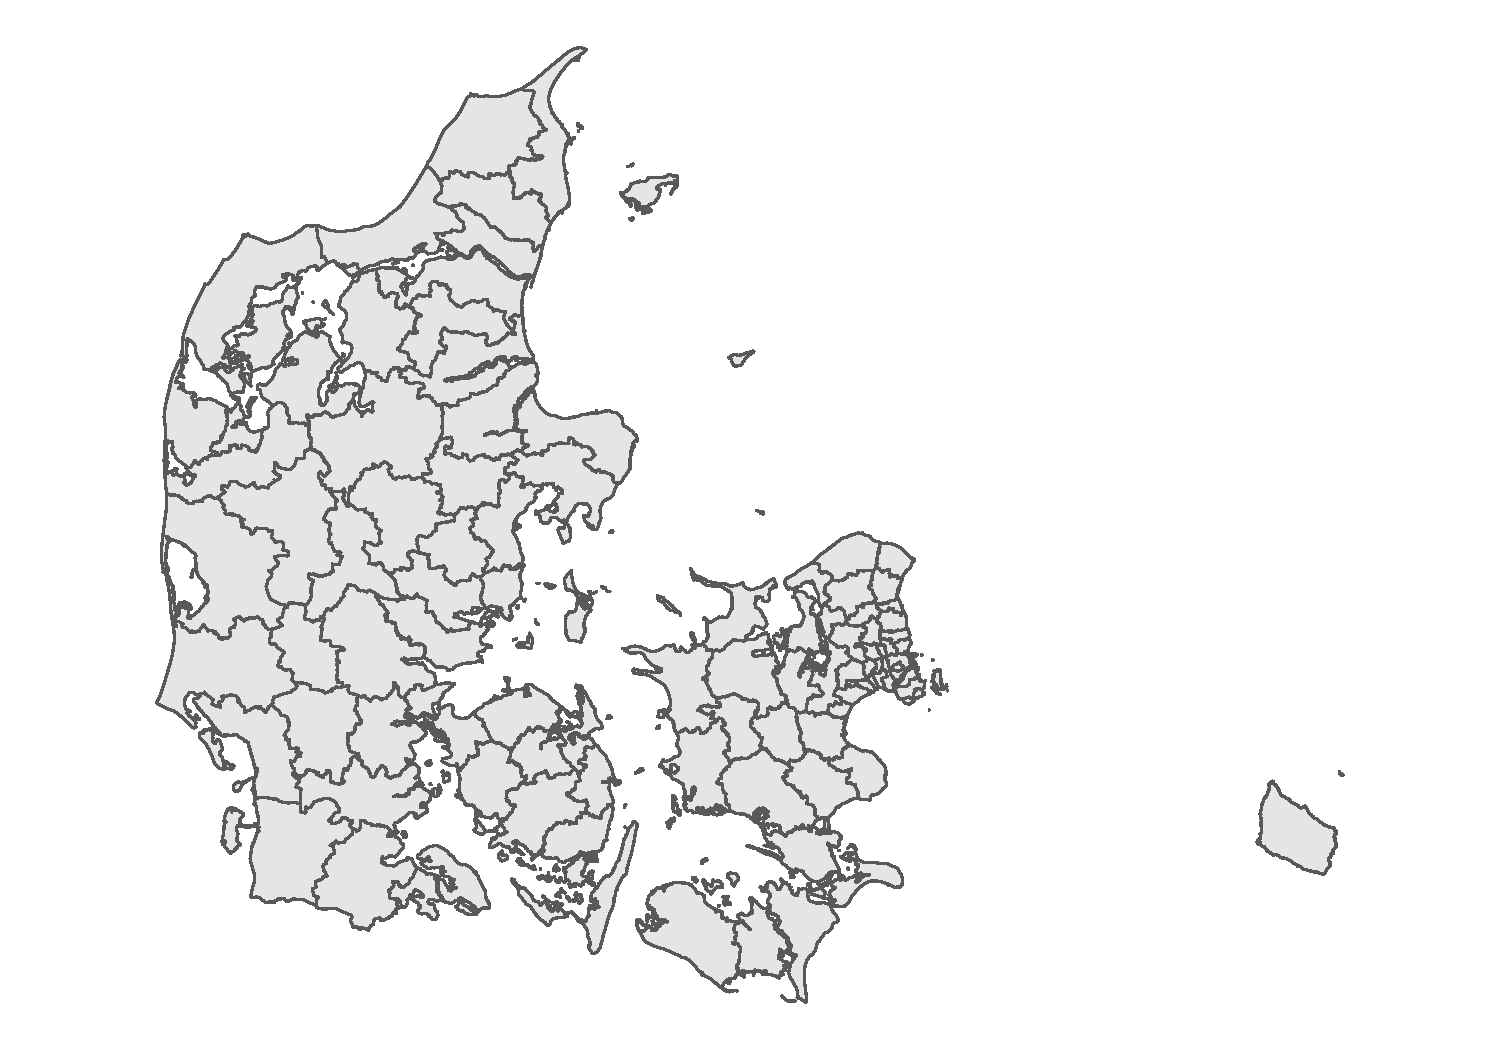
\includegraphics{crashcourse_slides_files/figure-beamer/unnamed-chunk-14-1.pdf}

\normalsize \columnsend
\end{frame}

\begin{frame}[fragile]{Fra geokodet til spatialt data}
\protect\hypertarget{fra-geokodet-til-spatialt-data}{}
\begin{itemize}
\item
  Tit har vi data (typisk \textbf{punkter}), som ikke er opbevaret som
  spatialt data men derimod blot med en række koordinater
\item
  Her skal vi transformere koordinaterne for at udnytte, at den
  underliggende information er spatial
\item
  Det kunne fx være nedenstånde datasæt over DSB-stationer:
\end{itemize}

\tiny

\begin{Shaded}
\begin{Highlighting}[]
\FunctionTok{library}\NormalTok{(janitor)}

\NormalTok{dsb }\OtherTok{\textless{}{-}}\NormalTok{ readxl}\SpecialCharTok{::}\FunctionTok{read\_xlsx}\NormalTok{(}\StringTok{"data/DSB\_Stations\_20201209.xlsm"}\NormalTok{) }\SpecialCharTok{\%\textgreater{}\%} 
  \FunctionTok{clean\_names}\NormalTok{() }\SpecialCharTok{\%\textgreater{}\%} 
  \FunctionTok{select}\NormalTok{(name, x, y)}

\FunctionTok{glimpse}\NormalTok{(dsb)}
\end{Highlighting}
\end{Shaded}

\begin{verbatim}
## Rows: 518
## Columns: 3
## $ name <chr> "Sommerland Sjælland", "Højby", "Nykøbing Sjælland", "Søborg", "S~
## $ x    <dbl> 12.024358, 11.603761, 11.672502, 12.333784, 11.711389, 12.513020,~
## $ y    <dbl> 55.54929, 55.91084, 55.92151, 56.10049, 55.54498, 55.77054, 55.77~
\end{verbatim}

\normalsize
\end{frame}

\begin{frame}[fragile]{Fra geokodet til spatialt data}
\protect\hypertarget{fra-geokodet-til-spatialt-data-1}{}
\begin{itemize}
\tightlist
\item
  Det er let at konvertere dette ``rå'' data til noget, \texttt{R}
  betragter som spatialt:
\end{itemize}

\tiny

\begin{Shaded}
\begin{Highlighting}[]
\CommentTok{\# fjern stationer uden koordinater}
\NormalTok{dsb }\OtherTok{\textless{}{-}}\NormalTok{ dsb }\SpecialCharTok{\%\textgreater{}\%} 
  \FunctionTok{filter}\NormalTok{(}\SpecialCharTok{!}\FunctionTok{is.na}\NormalTok{(x) }\SpecialCharTok{\&} \SpecialCharTok{!}\FunctionTok{is.na}\NormalTok{(y))}

\CommentTok{\# konverter til spatialt format}
\NormalTok{dsb }\OtherTok{\textless{}{-}}\NormalTok{ dsb }\SpecialCharTok{\%\textgreater{}\%} 
  \FunctionTok{st\_as\_sf}\NormalTok{(}\AttributeTok{coords =} \FunctionTok{c}\NormalTok{(}\StringTok{"x"}\NormalTok{, }\StringTok{"y"}\NormalTok{),}
           \AttributeTok{crs =} \DecValTok{4326}\NormalTok{)}

\FunctionTok{glimpse}\NormalTok{(dsb)}
\end{Highlighting}
\end{Shaded}

\begin{verbatim}
## Rows: 515
## Columns: 2
## $ name     <chr> "Sommerland Sjælland", "Højby", "Nykøbing Sjælland", "Søborg"~
## $ geometry <POINT [°]> POINT (12.02436 55.54929), POINT (11.60376 55.91084), P~
\end{verbatim}

\normalsize
\end{frame}

\hypertarget{visualisering-med-ggplot2}{%
\section{\texorpdfstring{Visualisering med
\{\texttt{ggplot2}\}}{Visualisering med \{ggplot2\}}}\label{visualisering-med-ggplot2}}

\begin{frame}[fragile]{Visualisering med \{\texttt{ggplot2}\}}
\protect\hypertarget{visualisering-med-ggplot2-1}{}
\begin{itemize}
\item
  Lad os prøve at se nærmere på vælgeropbakningen til Venstre ved
  forrige kommunalvalg
\item
  Jeg har snydt lidt hjemmefra og samlet et datasæt over stemmeandel på
  kommuneniveau:
\end{itemize}

\tiny

\begin{Shaded}
\begin{Highlighting}[]
\NormalTok{vshare }\OtherTok{\textless{}{-}} \FunctionTok{st\_read}\NormalTok{(}\AttributeTok{dsn =} \StringTok{"data/kommuner\_98"}\NormalTok{,}
                  \AttributeTok{layer =} \StringTok{"kommuner\_98"}\NormalTok{)}
\end{Highlighting}
\end{Shaded}

\normalsize

\tiny

\begin{Shaded}
\begin{Highlighting}[]
\FunctionTok{head}\NormalTok{(vshare)}
\end{Highlighting}
\end{Shaded}

\begin{verbatim}
## Simple feature collection with 6 features and 7 fields
## Geometry type: MULTIPOLYGON
## Dimension:     XY
## Bounding box:  xmin: 12.2635 ymin: 55.53633 xmax: 12.73425 ymax: 55.77944
## Geodetic CRS:  WGS 84
##   dagi_id          navn kommune_nr             region party  total      share
## 1  389103     København        101 Region Hovedstaden 23652 300216 0.07878328
## 2  389104 Frederiksberg        147 Region Hovedstaden  3748  59298 0.06320618
## 3  389105      Ballerup        151 Region Hovedstaden  2739  25949 0.10555320
## 4  389106       Brøndby        153 Region Hovedstaden  1689  16921 0.09981680
## 5  389107        Dragør        155 Region Hovedstaden  1732   8403 0.20611686
## 6  389108      Gentofte        157 Region Hovedstaden  2649  40430 0.06552065
##                         geometry
## 1 MULTIPOLYGON (((12.54502 55...
## 2 MULTIPOLYGON (((12.53735 55...
## 3 MULTIPOLYGON (((12.3423 55....
## 4 MULTIPOLYGON (((12.44279 55...
## 5 MULTIPOLYGON (((12.64513 55...
## 6 MULTIPOLYGON (((12.59175 55...
\end{verbatim}

\normalsize
\end{frame}

\begin{frame}[fragile]{Visualisering med \{\texttt{ggplot2}\}}
\protect\hypertarget{visualisering-med-ggplot2-2}{}
\columnsbegin
\column{.5\textwidth}

\tiny

\begin{Shaded}
\begin{Highlighting}[]
\FunctionTok{ggplot}\NormalTok{() }\SpecialCharTok{+}
  \FunctionTok{geom\_sf}\NormalTok{(}\AttributeTok{data =}\NormalTok{ vshare)}
\end{Highlighting}
\end{Shaded}

\normalsize \column{.5\textwidth}

\tiny

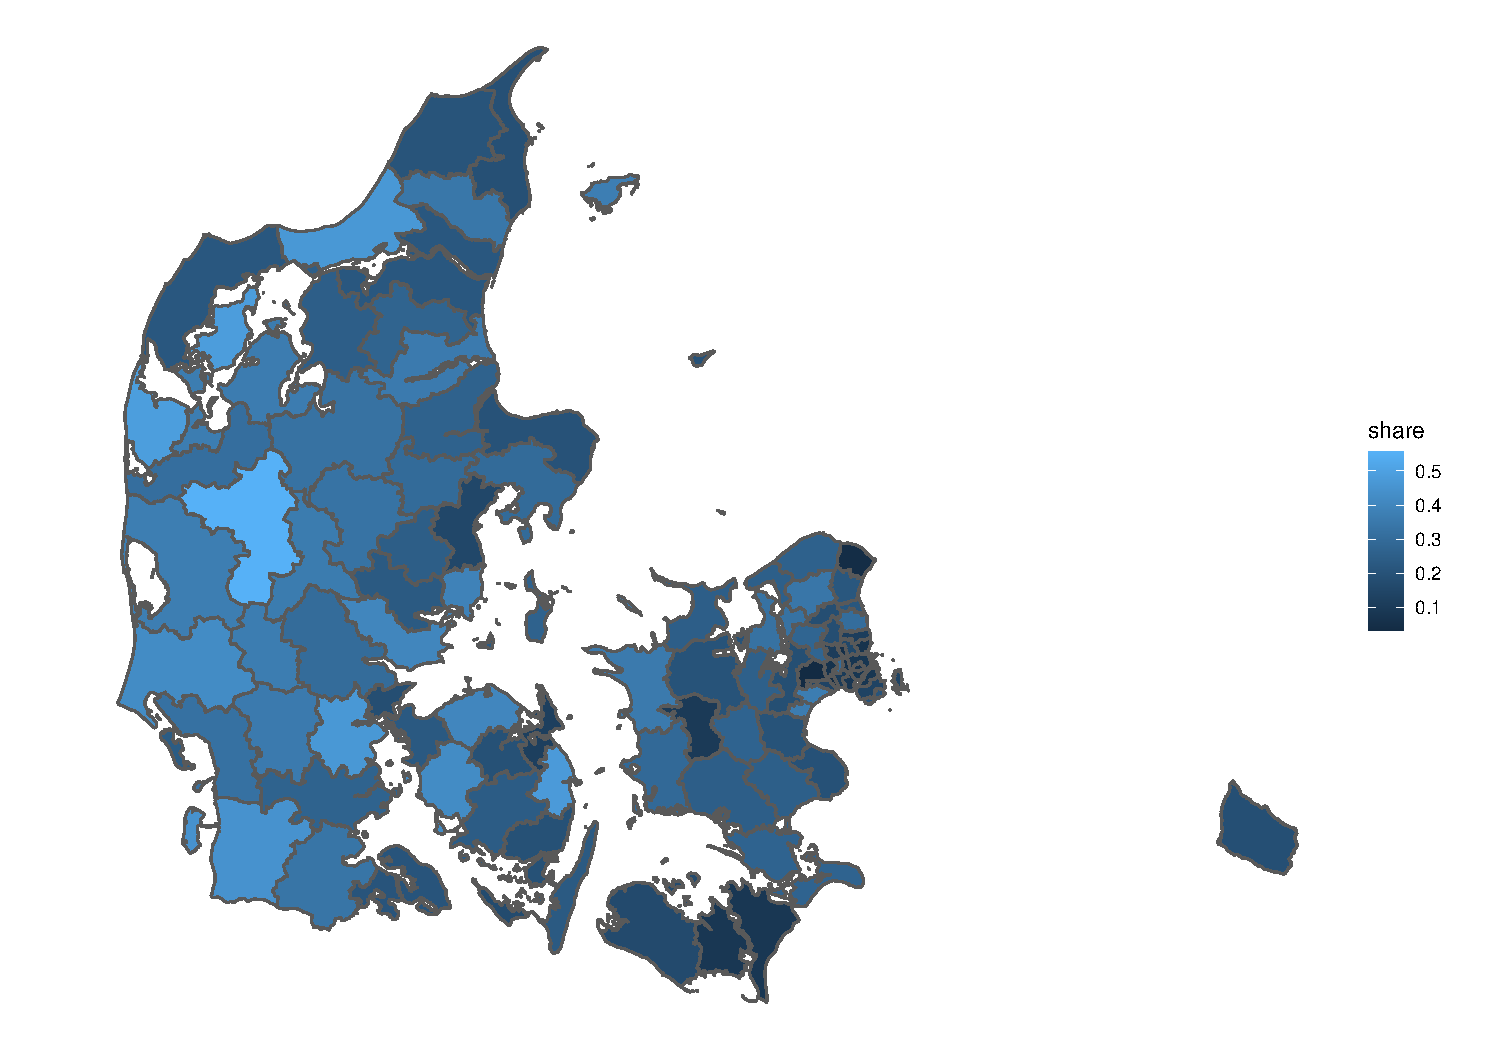
\includegraphics{crashcourse_slides_files/figure-beamer/unnamed-chunk-20-1.pdf}

\normalsize \columnsend
\end{frame}

\begin{frame}[fragile]{Visualisering med \{\texttt{ggplot2}\}}
\protect\hypertarget{visualisering-med-ggplot2-3}{}
\columnsbegin
\column{.5\textwidth}

\tiny

\begin{Shaded}
\begin{Highlighting}[]
\FunctionTok{ggplot}\NormalTok{() }\SpecialCharTok{+}
  \FunctionTok{geom\_sf}\NormalTok{(}\AttributeTok{data =}\NormalTok{ vshare) }\SpecialCharTok{+}
  \FunctionTok{theme\_void}\NormalTok{()}
\end{Highlighting}
\end{Shaded}

\normalsize \column{.5\textwidth}

\tiny

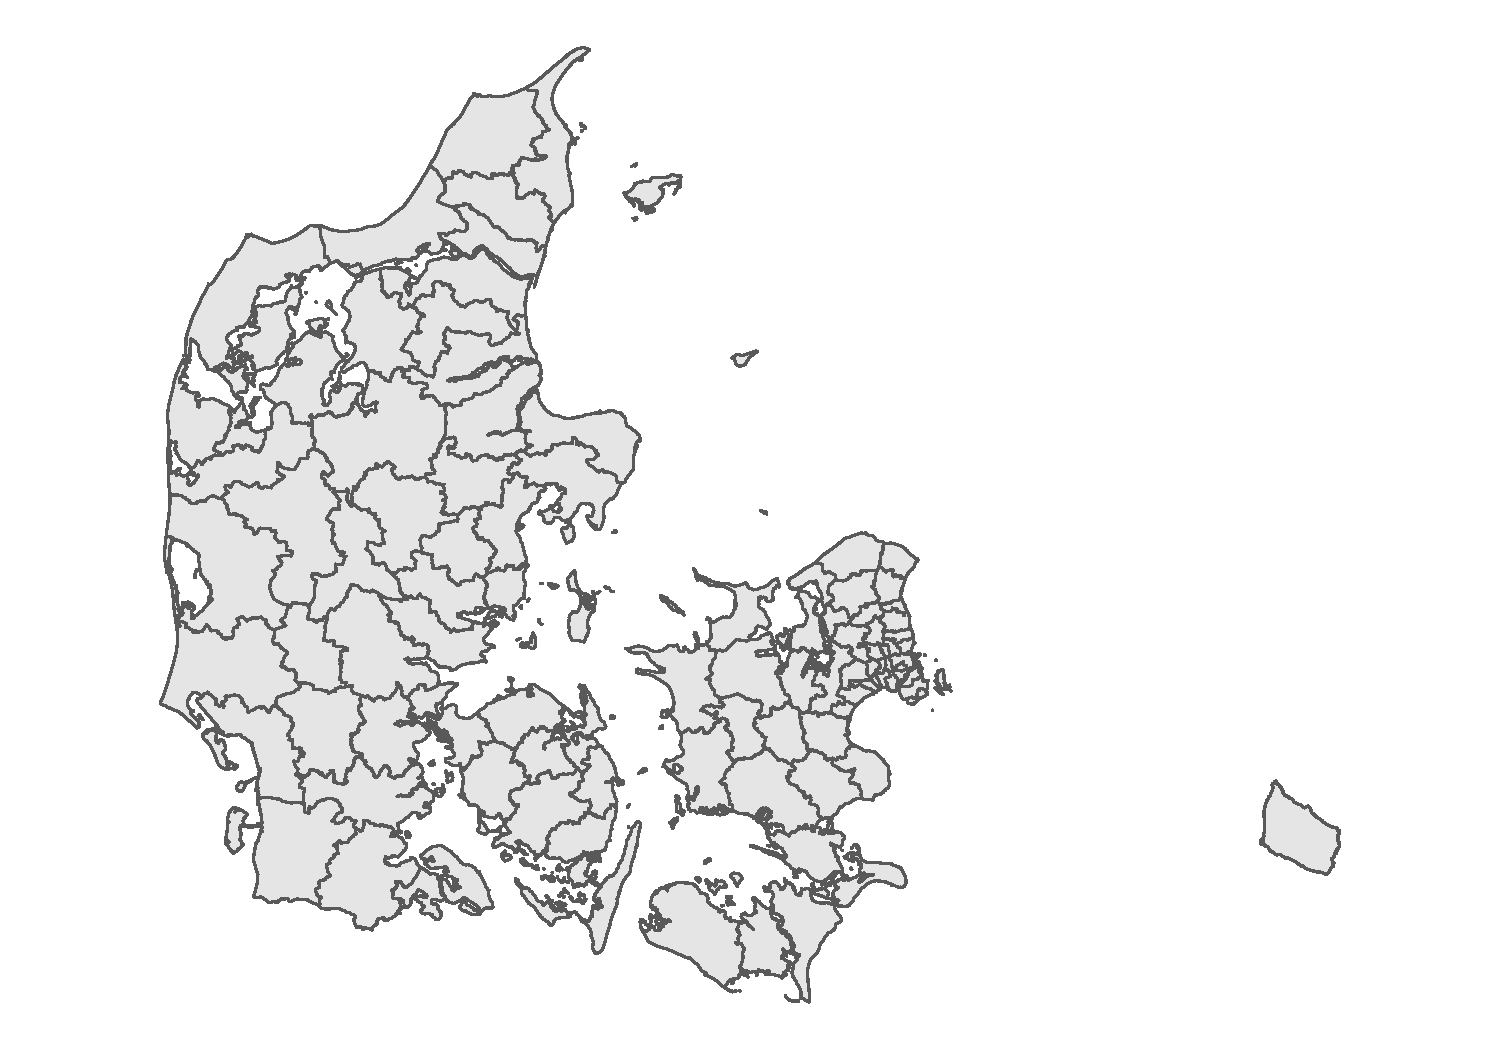
\includegraphics{crashcourse_slides_files/figure-beamer/unnamed-chunk-22-1.pdf}

\normalsize \columnsend
\end{frame}

\begin{frame}[fragile]{Visualisering med \{\texttt{ggplot2}\}}
\protect\hypertarget{visualisering-med-ggplot2-4}{}
\columnsbegin
\column{.5\textwidth}

\tiny

\begin{Shaded}
\begin{Highlighting}[]
\FunctionTok{ggplot}\NormalTok{() }\SpecialCharTok{+}
  \FunctionTok{geom\_sf}\NormalTok{(}\AttributeTok{data =}\NormalTok{ vshare,}
          \FunctionTok{aes}\NormalTok{(}\AttributeTok{fill =}\NormalTok{ share)) }\SpecialCharTok{+}
  \FunctionTok{theme\_void}\NormalTok{()}
\end{Highlighting}
\end{Shaded}

\normalsize \column{.5\textwidth}

\tiny

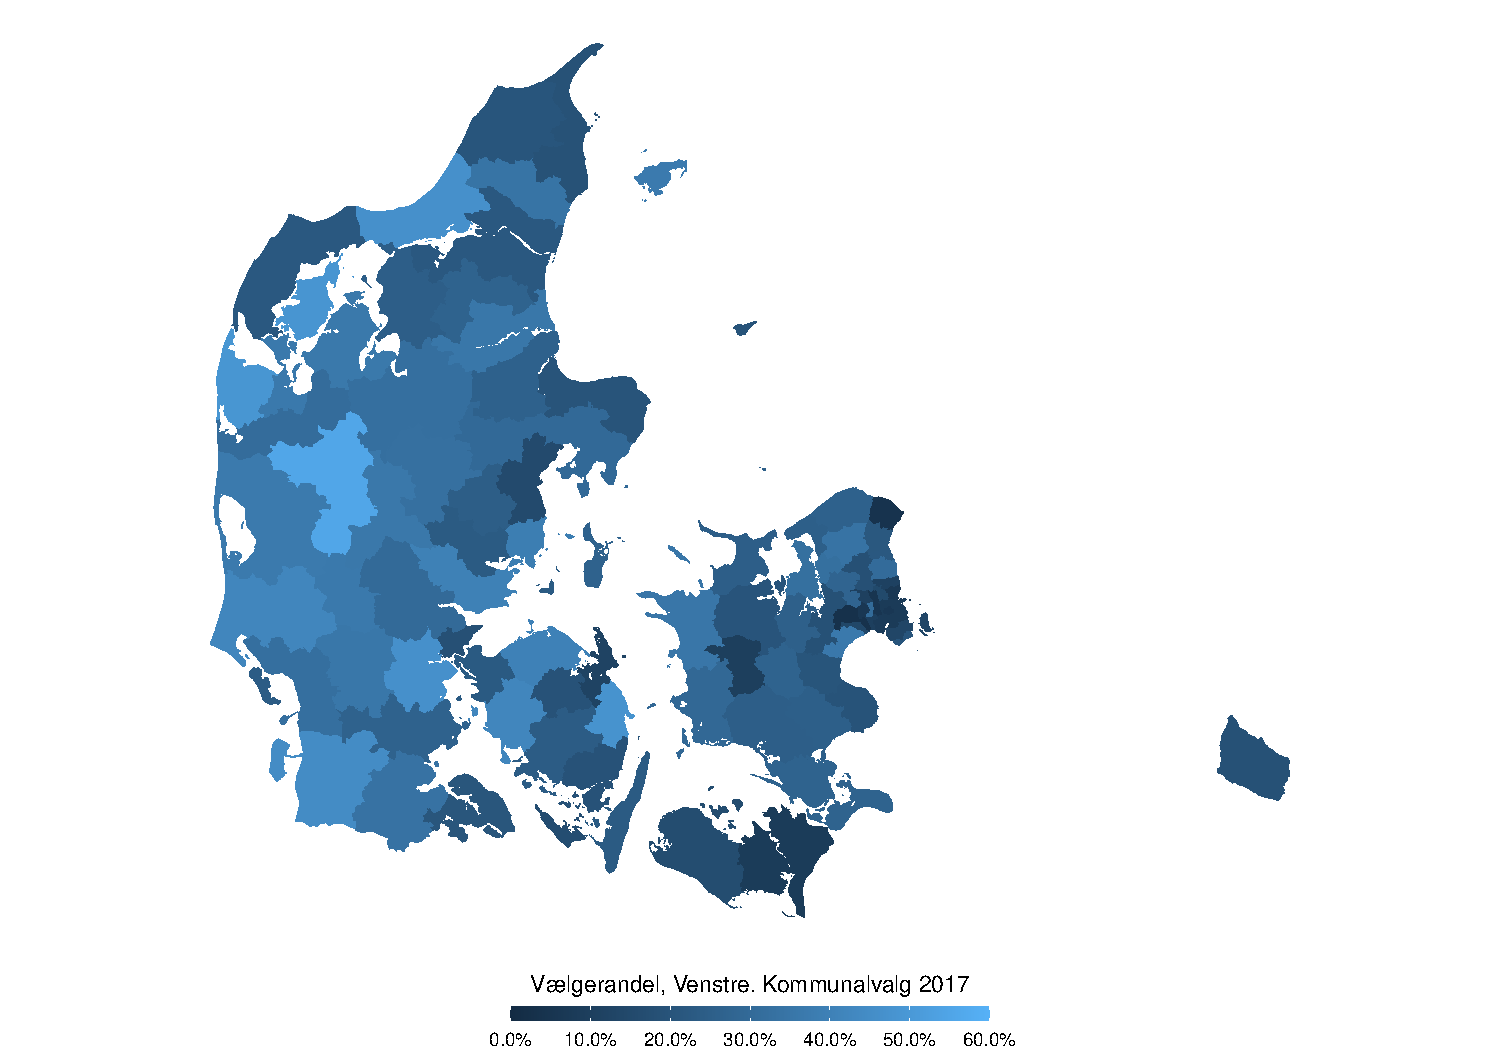
\includegraphics{crashcourse_slides_files/figure-beamer/unnamed-chunk-24-1.pdf}

\normalsize \columnsend
\end{frame}

\begin{frame}[fragile]{Visualisering med \{\texttt{ggplot2}\}}
\protect\hypertarget{visualisering-med-ggplot2-5}{}
\columnsbegin
\column{.5\textwidth}

\tiny

\begin{Shaded}
\begin{Highlighting}[]
\FunctionTok{ggplot}\NormalTok{() }\SpecialCharTok{+}
  \FunctionTok{geom\_sf}\NormalTok{(}\AttributeTok{data =}\NormalTok{ vshare,}
          \FunctionTok{aes}\NormalTok{(}\AttributeTok{fill =}\NormalTok{ share),}
          \AttributeTok{color =} \StringTok{"transparent"}\NormalTok{) }\SpecialCharTok{+}
  \FunctionTok{theme\_void}\NormalTok{()}
\end{Highlighting}
\end{Shaded}

\normalsize \column{.5\textwidth}

\tiny

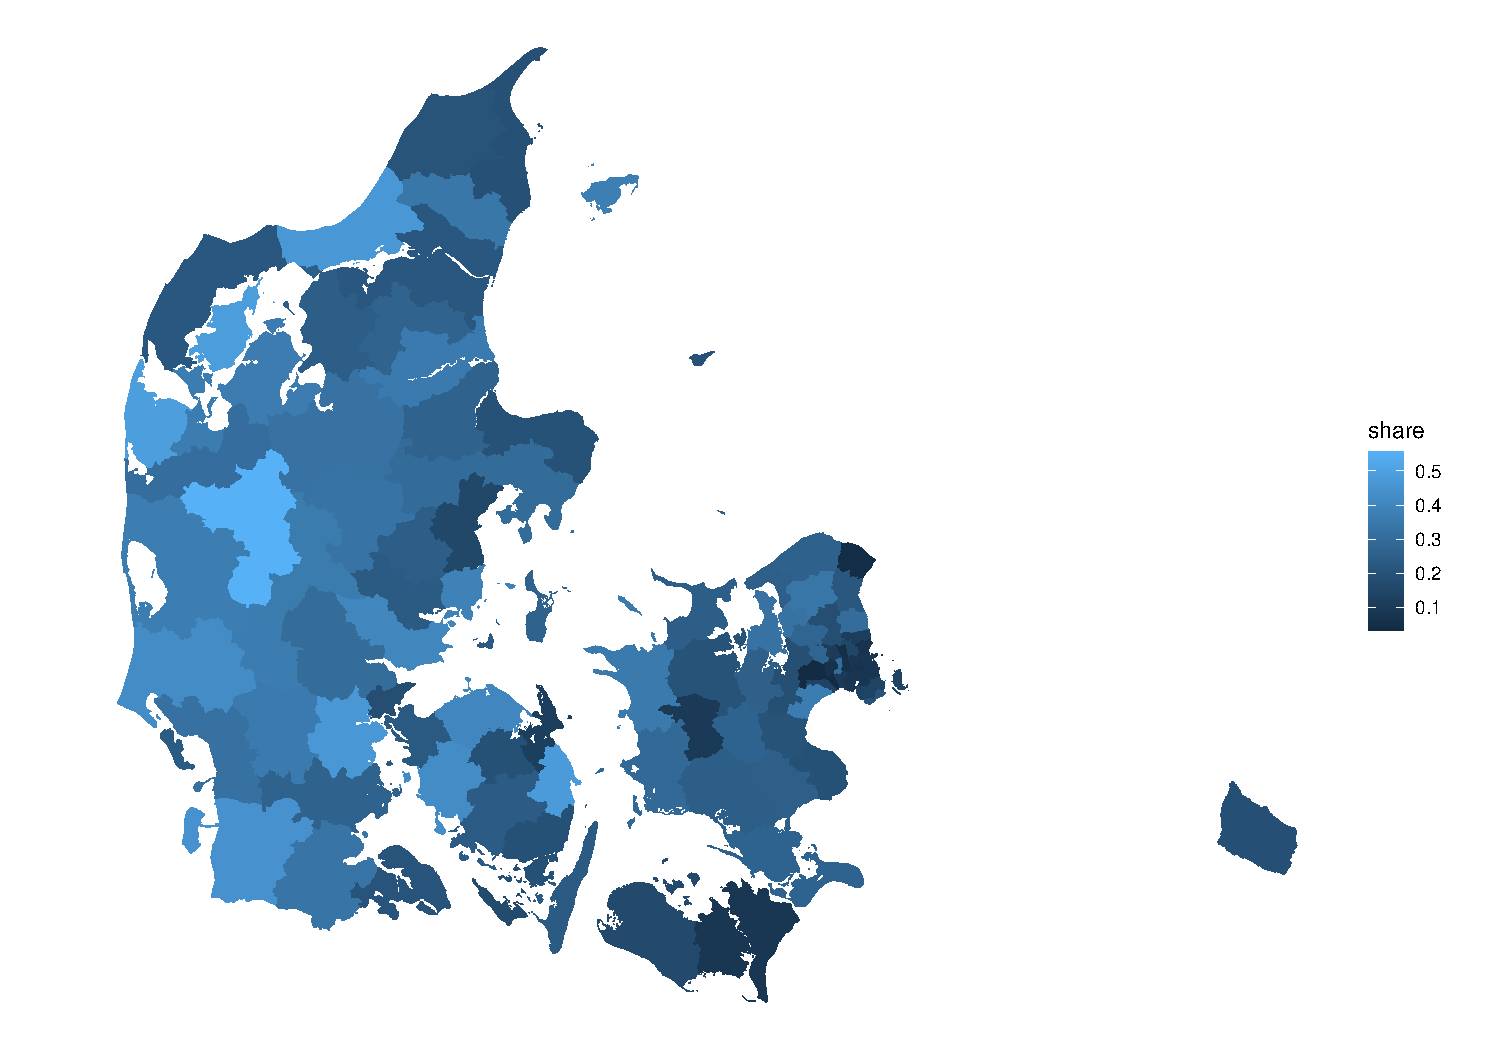
\includegraphics{crashcourse_slides_files/figure-beamer/unnamed-chunk-26-1.pdf}

\normalsize \columnsend
\end{frame}

\begin{frame}[fragile]{Visualisering med \{\texttt{ggplot2}\}}
\protect\hypertarget{visualisering-med-ggplot2-6}{}
\columnsbegin
\column{.5\textwidth}

\tiny

\begin{Shaded}
\begin{Highlighting}[]
\FunctionTok{ggplot}\NormalTok{() }\SpecialCharTok{+}
  \FunctionTok{geom\_sf}\NormalTok{(}\AttributeTok{data =}\NormalTok{ vshare,}
          \FunctionTok{aes}\NormalTok{(}\AttributeTok{fill =}\NormalTok{ share),}
          \AttributeTok{color =} \StringTok{"transparent"}\NormalTok{) }\SpecialCharTok{+}
  \FunctionTok{scale\_fill\_continuous}\NormalTok{(}\AttributeTok{name =} \StringTok{"Vælgerandel, Venstre. Kommunalvalg 2017"}\NormalTok{,}
                        \AttributeTok{labels =}\NormalTok{ scales}\SpecialCharTok{::}\NormalTok{percent,}
                        \AttributeTok{breaks =} \FunctionTok{seq}\NormalTok{(}\DecValTok{0}\NormalTok{, }\FloatTok{0.6}\NormalTok{, .}\DecValTok{1}\NormalTok{),}
                        \AttributeTok{limits =} \FunctionTok{c}\NormalTok{(}\DecValTok{0}\NormalTok{, .}\DecValTok{6}\NormalTok{)) }\SpecialCharTok{+}
  \FunctionTok{theme\_void}\NormalTok{() }\SpecialCharTok{+}
  \FunctionTok{theme}\NormalTok{(}\AttributeTok{legend.position =} \StringTok{"bottom"}\NormalTok{) }\SpecialCharTok{+}
  \FunctionTok{guides}\NormalTok{(}\AttributeTok{fill =} \FunctionTok{guide\_colorbar}\NormalTok{(}\AttributeTok{title.position =} \StringTok{"top"}\NormalTok{,}
                               \AttributeTok{title.hjust =}\NormalTok{ .}\DecValTok{5}\NormalTok{,}
                               \AttributeTok{barwidth =} \DecValTok{16}\NormalTok{,}
                               \AttributeTok{barheight =}\NormalTok{ .}\DecValTok{5}\NormalTok{))}
\end{Highlighting}
\end{Shaded}

\normalsize \column{.5\textwidth}

\tiny

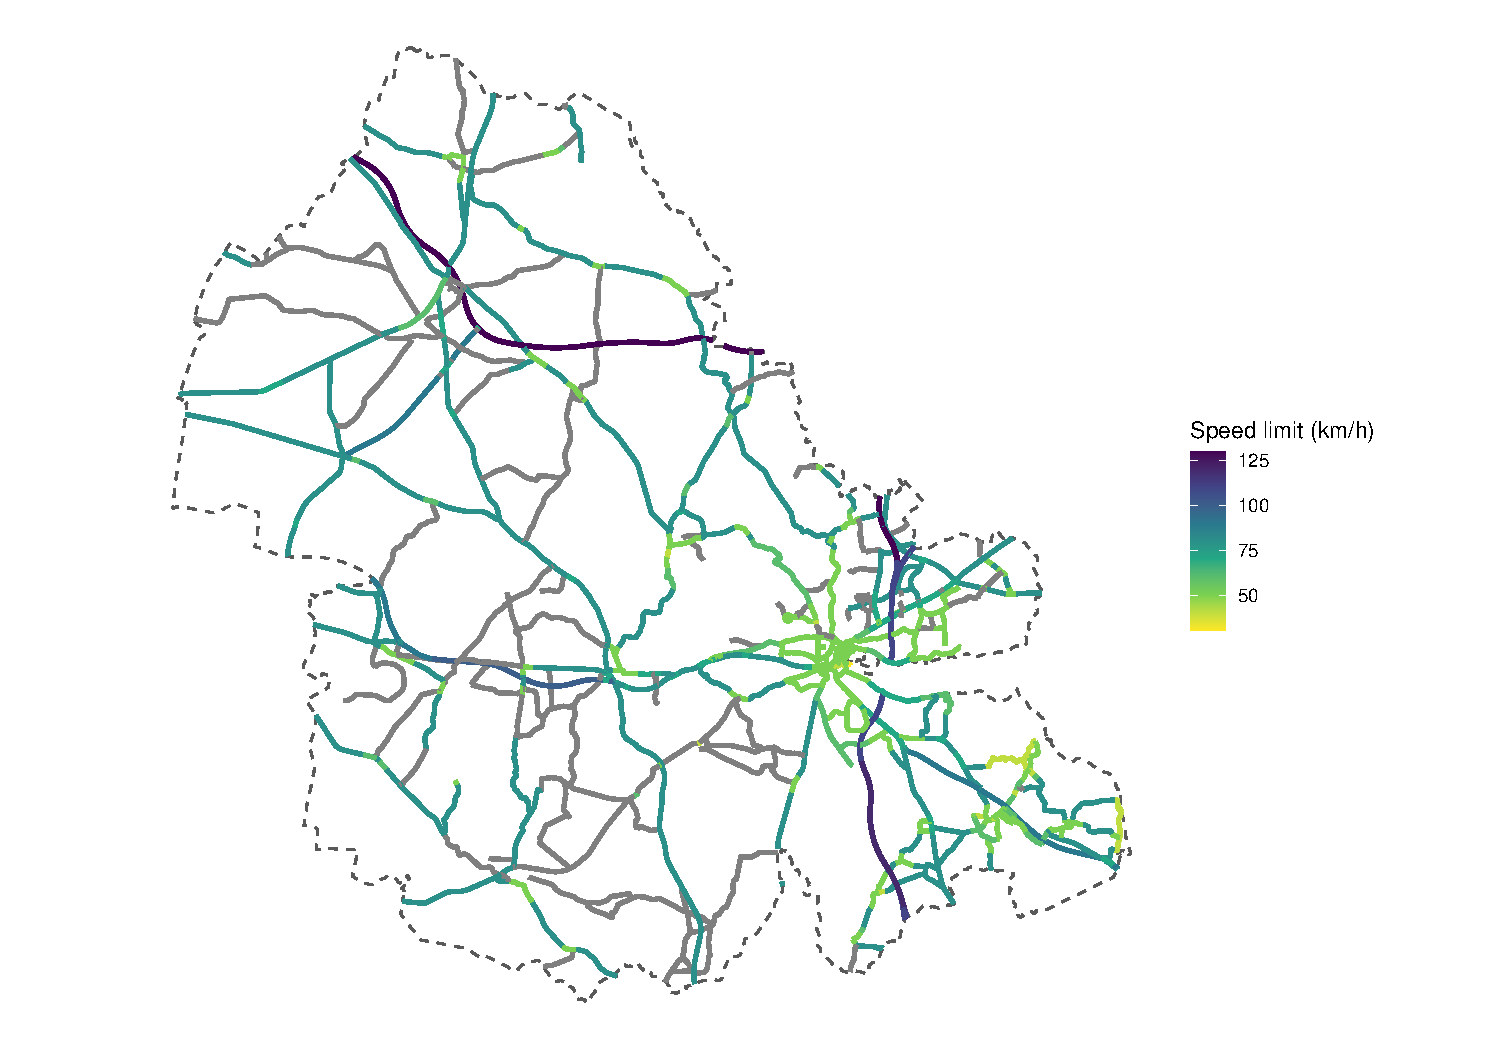
\includegraphics{crashcourse_slides_files/figure-beamer/unnamed-chunk-28-1.pdf}

\normalsize

\columnsend
\end{frame}

\hypertarget{interaktiv-visualisering-med-tmap}{%
\section{\texorpdfstring{Interaktiv visualisering med
\{\texttt{tmap}\}}{Interaktiv visualisering med \{tmap\}}}\label{interaktiv-visualisering-med-tmap}}

\begin{frame}[fragile]{Interaktiv visualisering med \{\texttt{tmap}\}}
\protect\hypertarget{interaktiv-visualisering-med-tmap-1}{}
\begin{itemize}
\item
  \texttt{tmap} er nyeste skud på stammen, når det kommer til at
  visualisere geospatial data. I modsætning til \texttt{ggplot2} er
  pakken udviklet \emph{specifikt} til dette formål
\item
  \texttt{tmap}-pakken er ikke helt lige så fleksibel som
  \texttt{ggplot2}. Der skal lige mere arbejde til for at gøre dit plot
  pænt. Derudover minder syntaxen meget om
\item
  Til gengæld er \texttt{tmap} eminent til at generere
  \textbf{interaktive kort}!
\item
  Af samme grund bruger jeg den ofte, når jeg arbejder \emph{med} data.
  Det gør det nemt at inspicere dine datasæt
\end{itemize}
\end{frame}

\begin{frame}[fragile]{Interaktiv visualisering med \{\texttt{tmap}\}}
\protect\hypertarget{interaktiv-visualisering-med-tmap-2}{}
\columnsbegin
\column{.5\textwidth}

\tiny

\begin{Shaded}
\begin{Highlighting}[]
\FunctionTok{library}\NormalTok{(tmap)}

\FunctionTok{tmap\_mode}\NormalTok{(}\StringTok{"view"}\NormalTok{)}

\FunctionTok{tm\_shape}\NormalTok{(vshare) }\SpecialCharTok{+}
  \FunctionTok{tm\_polygons}\NormalTok{(}\AttributeTok{col =} \StringTok{"share"}\NormalTok{)}
\end{Highlighting}
\end{Shaded}

\normalsize \column{.5\textwidth}

\begin{figure}[H]
    \centering
    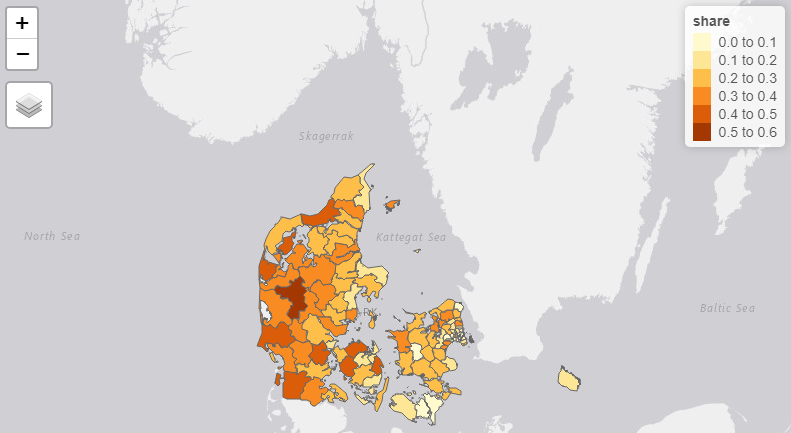
\includegraphics[width=.90\textwidth]{pictures/tmap.png}
\end{figure}

\columnsend
\end{frame}

\hypertarget{datakilder}{%
\section{Datakilder}\label{datakilder}}

\begin{frame}{DAGI}
\protect\hypertarget{dagi}{}
\columnsbegin

\column{.6\textwidth}

\begin{itemize}
\tightlist
\item
  \emph{``\textbf{Danmarks Administrative Geografiske Inddeling (DAGI)}
  beskriver landets administrative og geografiske inddeling i kommuner,
  regioner, sogne, retskredse, politikredse, postnumre,
  opstillingskredse og lignende.''} --
  \href{https://dawadocs.dataforsyningen.dk/dok/dagi}{DAWA}
\end{itemize}

\medskip

\begin{itemize}
\item
  \ldots{} med andre ord; alt hvad vi kunne drømme om
\item
  DAGI-data kan hentes via Styrelsen for Dataforsyning og
  Effektiviserings
  \href{https://datafordeler.dk/dataoversigt/}{Datafordeler}
\item
  Det er en ret håbløs hjemmeside, til gengæld er der masser at vælge
  mellem (inkl. historiske enheder!)
\end{itemize}

\column{.4\textwidth}

\begin{figure}[H]
    \centering
    
\includegraphics[width=.90\textwidth]{pictures/logo_sdfe.png}
\end{figure}

\columnsend
\end{frame}

\begin{frame}{DAGI}
\protect\hypertarget{dagi-1}{}
\begin{itemize}
\item
  Til de fleste formål kan vi hoppe uden om Datafordelen ved at bruge
  \href{https://dawadocs.dataforsyningen.dk/dok/dagi}{DAWA (Danmarks
  Adressers Web API)} og den
  \href{https://dawadocs.dataforsyningen.dk/dok/api\#dagi}{tilhørende
  API}
\item
  API'en er plug 'n play, hvor vi kan vælge de
  \textcolor{purple}{enheder}, vi skal bruge, og specificere
  \textcolor{teal}{format}:
\item
  \nolinkurl{https://api.dataforsyningen.dk/ \textcolor{purple}{kommuner}?format=\textcolor{teal}{geojson}}
\end{itemize}
\end{frame}

\begin{frame}[fragile]{DAGI: et eksempel}
\protect\hypertarget{dagi-et-eksempel}{}
\columnsbegin
\column{.5\textwidth}

\tiny

\begin{Shaded}
\begin{Highlighting}[]
\CommentTok{\# definér data}
\NormalTok{url }\OtherTok{\textless{}{-}} 
  \StringTok{"https://api.dataforsyningen.dk/kommuner?format=geojson"}

\CommentTok{\# indlæs data}
\NormalTok{kommuner\_raw }\OtherTok{\textless{}{-}} 
  \FunctionTok{read\_sf}\NormalTok{(url)}

\CommentTok{\# plot data}
\FunctionTok{ggplot}\NormalTok{() }\SpecialCharTok{+}
  \FunctionTok{geom\_sf}\NormalTok{(}\AttributeTok{data =}\NormalTok{ kommuner\_raw) }\SpecialCharTok{+}
  \FunctionTok{theme\_void}\NormalTok{()}
\end{Highlighting}
\end{Shaded}

\normalsize \column{.5\textwidth}

\tiny

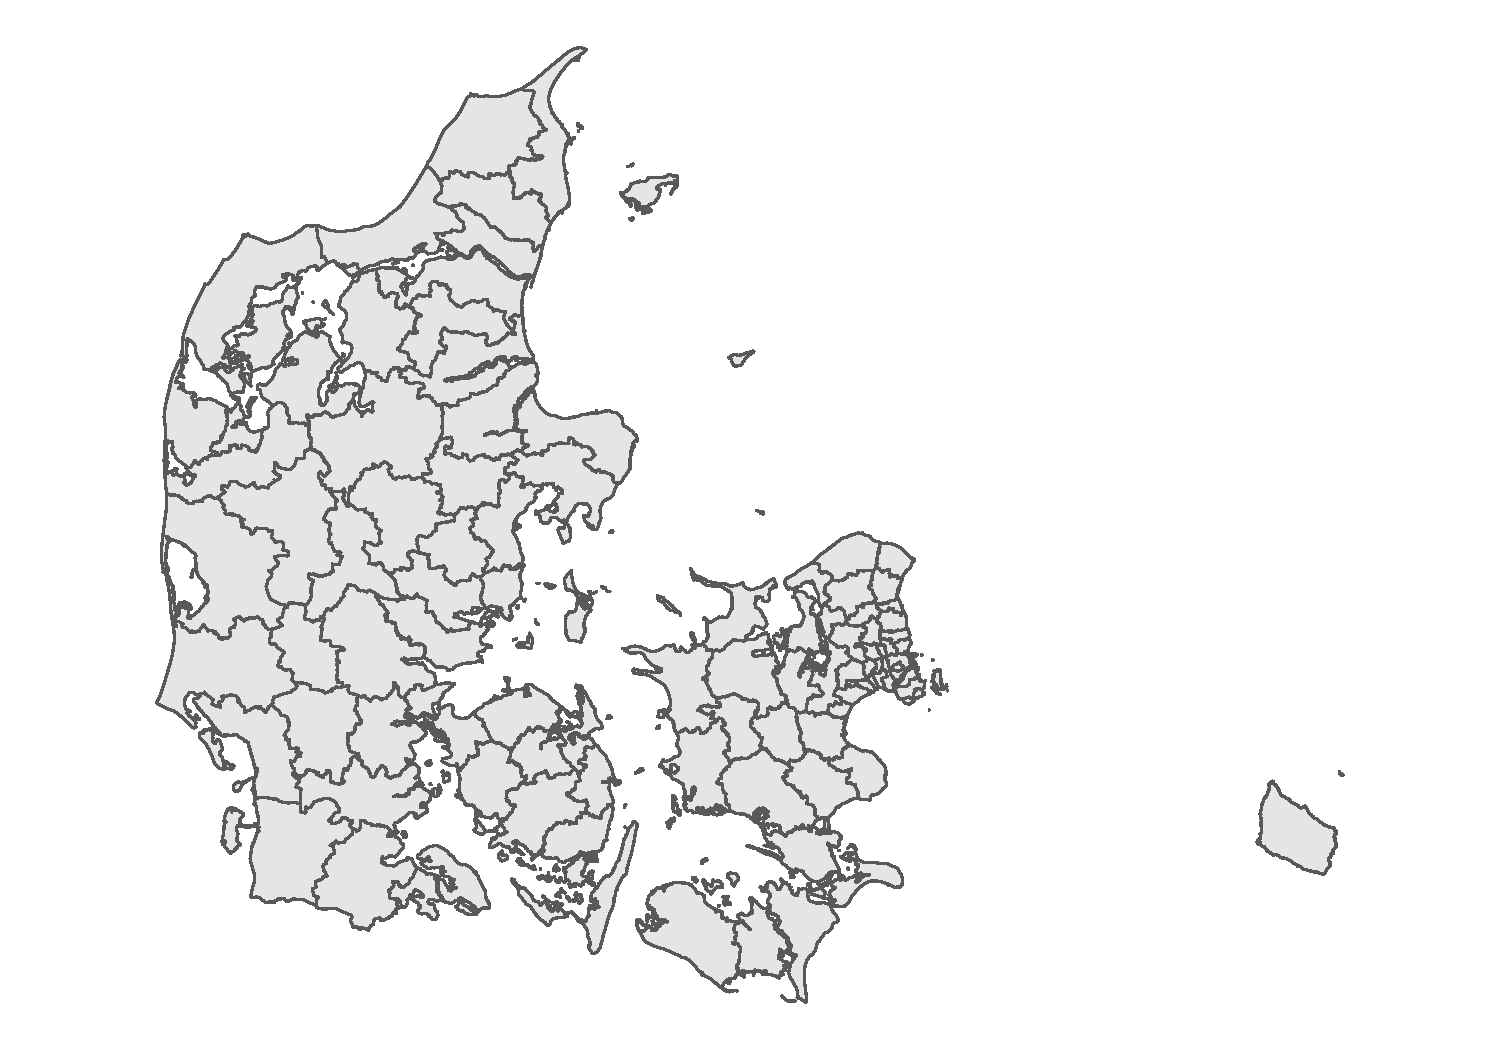
\includegraphics{crashcourse_slides_files/figure-beamer/unnamed-chunk-31-1.pdf}

\normalsize \columnsend
\end{frame}

\begin{frame}{OpenStreetMap}
\protect\hypertarget{openstreetmap}{}
\columnsbegin

\column{.6\textwidth}

\begin{itemize}
\item
  \href{https://www.openstreetmap.org/about}{OpenStreetMap (OSM)} er en
  crowd sourced geografisk database med detaljeret information om hele
  verden
\item
  OSM indeholder data på (næsten) alt, hvad hjertet begærer
\item
  OSM har en tilhørende
  \href{https://wiki.openstreetmap.org/wiki/Map_features}{wiki}, med en
  oversigt over de forskellige features
\end{itemize}

\column{.4\textwidth}

\begin{figure}[H]
    \centering
    
\includegraphics[width=.75\textwidth]{pictures/Openstreetmap_logo.svg}
\end{figure}

\columnsend
\end{frame}

\begin{frame}[fragile]{OpenStreetMap}
\protect\hypertarget{openstreetmap-1}{}
\columnsbegin

\column{.6\textwidth}

\begin{itemize}
\item
  Vi kan bruge R-pakken
  \href{https://cran.r-project.org/web/packages/osmdata/vignettes/osmdata.html}{\{\texttt{osmdata}\}}
  til at hente OSM-data direkte i \texttt{R}
\item
  Her skal vi bruge

  \begin{itemize}
  \tightlist
  \item
    En geografisk afgrænsning
  \item
    Valg af features (vha. argumenterne \texttt{key} og \texttt{value}):
  \end{itemize}
\end{itemize}

\column{.4\textwidth}

\begin{figure}[H]
    \centering
    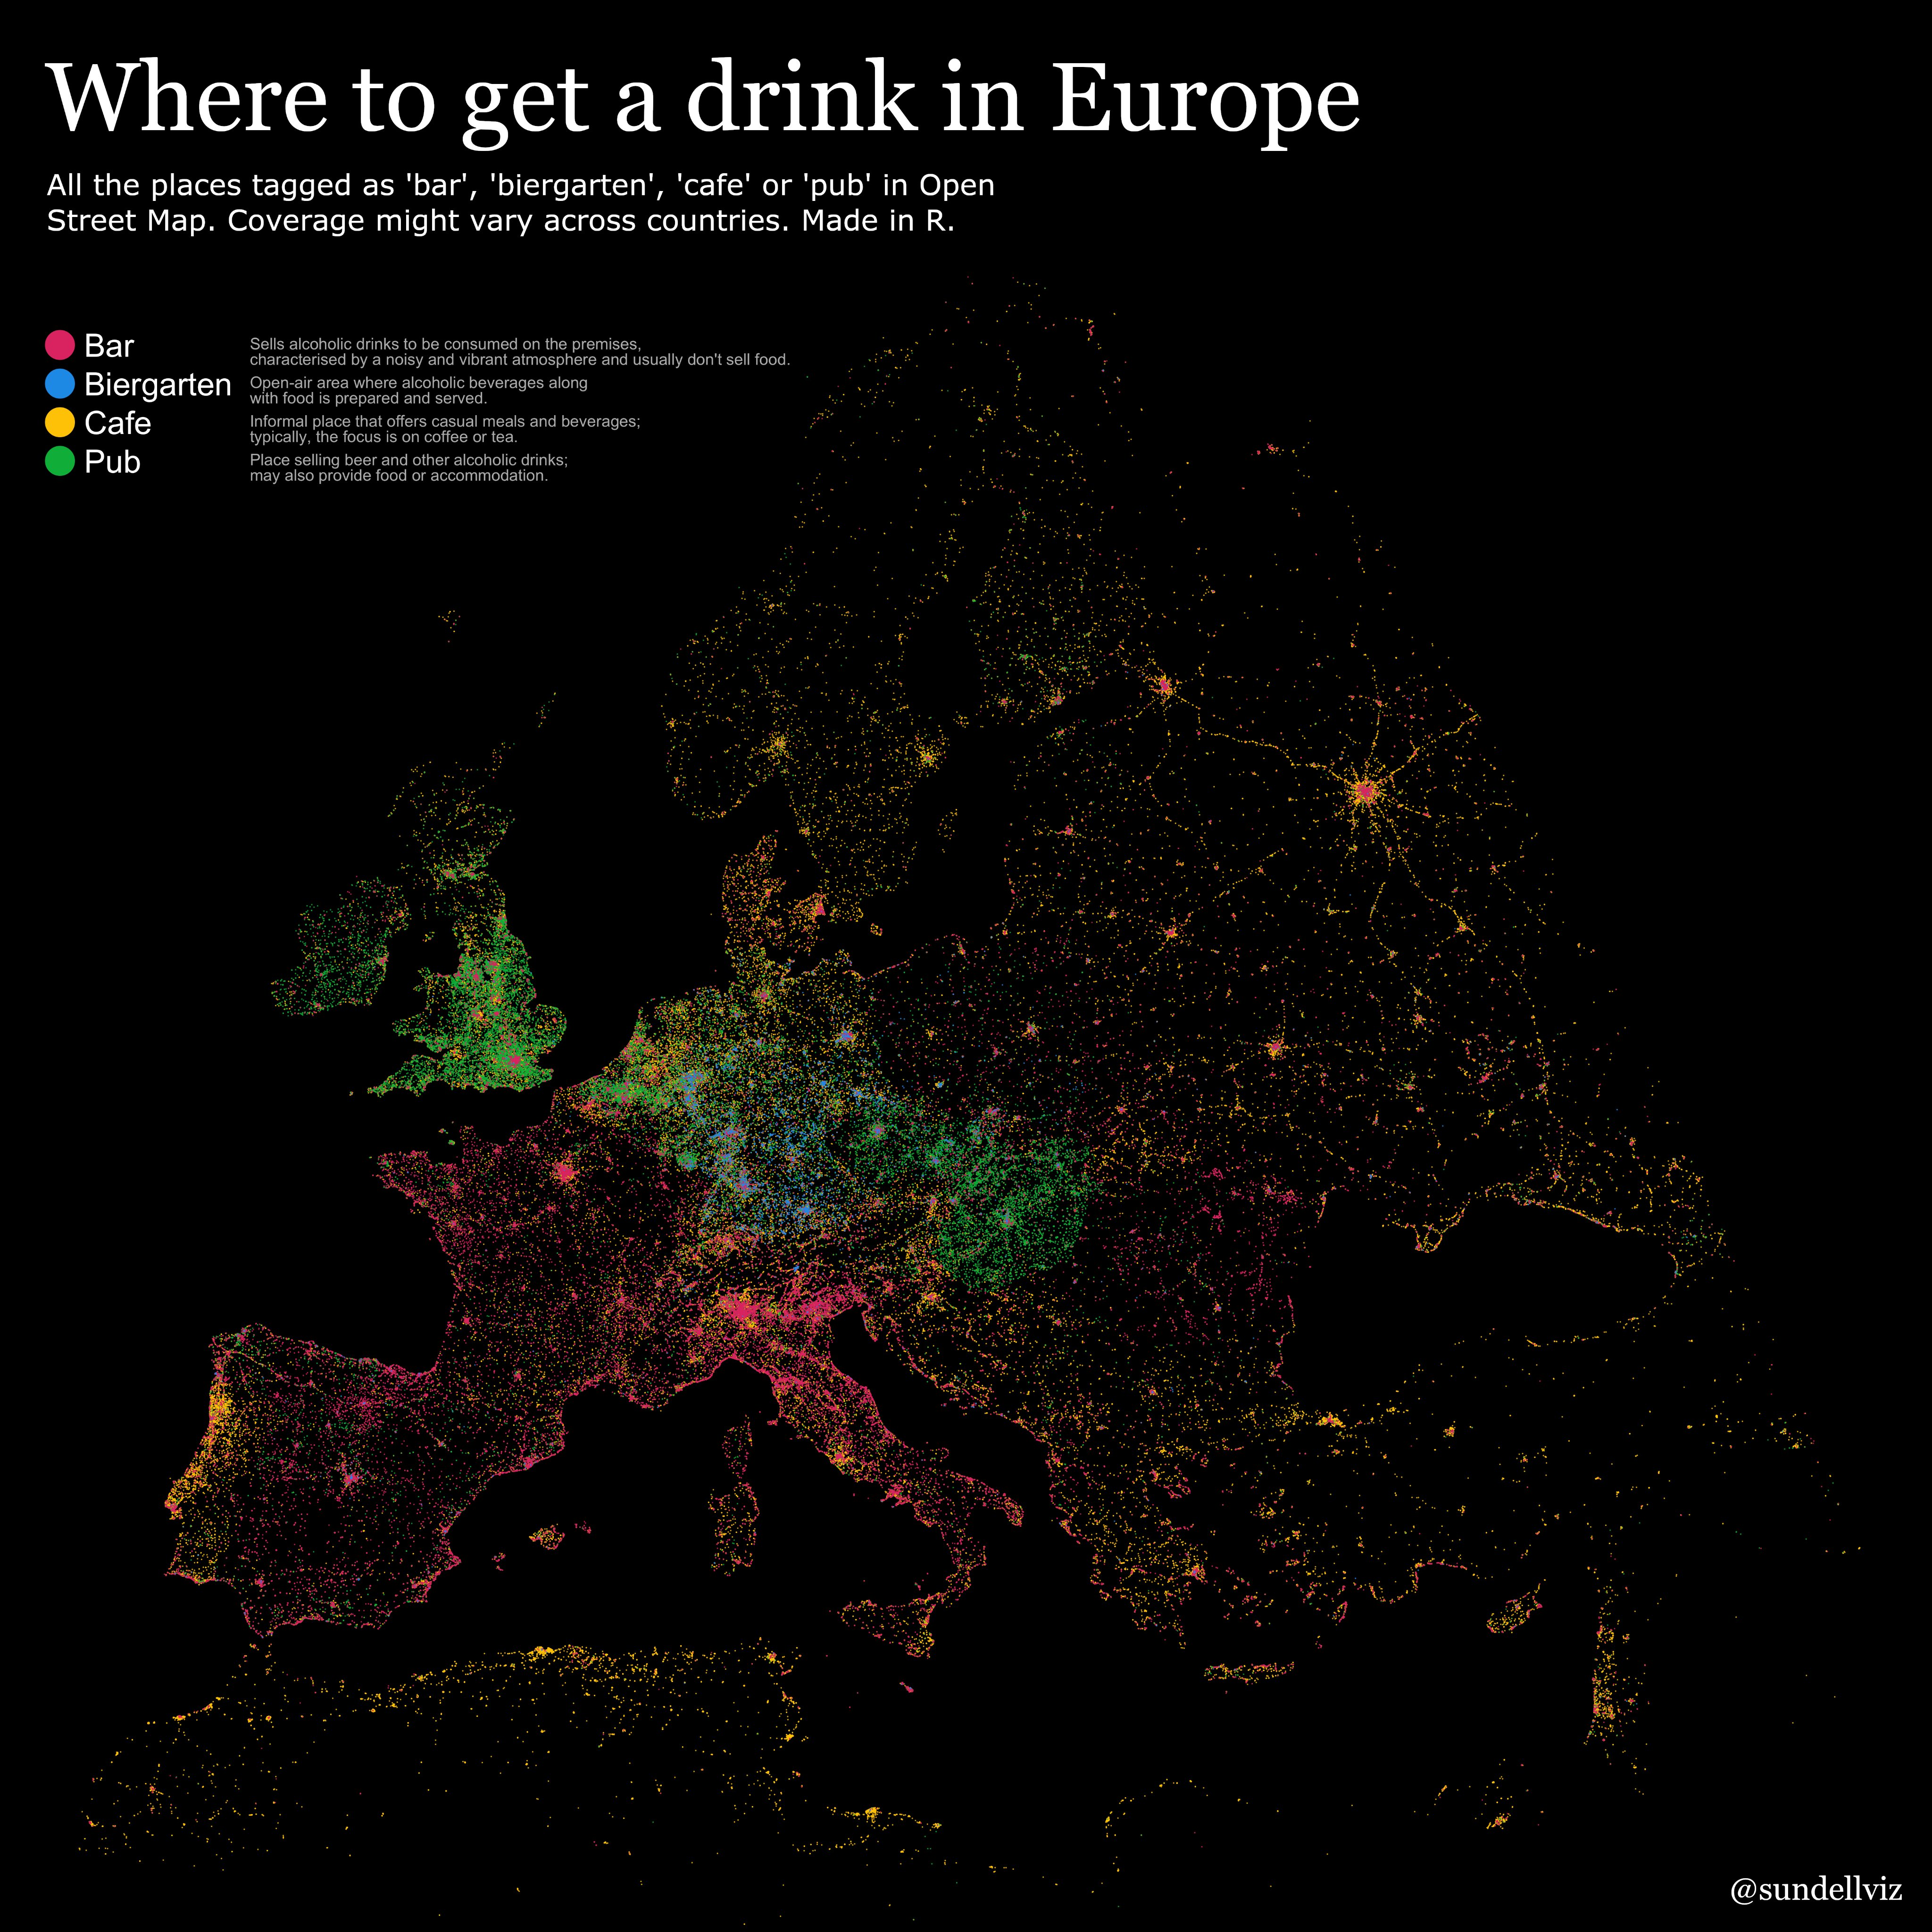
\includegraphics[width=.90\textwidth]{pictures/sundell_bars.png}
\end{figure}

\columnsend
\end{frame}

\begin{frame}[fragile]{OpenStreetMap: et eksempel}
\protect\hypertarget{openstreetmap-et-eksempel}{}
\columnsbegin
\column{.5\textwidth}

\tiny

\begin{Shaded}
\begin{Highlighting}[]
\FunctionTok{library}\NormalTok{(osmdata)}

\CommentTok{\# Hent OSM{-}data for Vejle}
\NormalTok{vejle }\OtherTok{\textless{}{-}}\NormalTok{ kommuner\_raw }\SpecialCharTok{\%\textgreater{}\%} 
  \FunctionTok{filter}\NormalTok{(navn }\SpecialCharTok{==} \StringTok{"Vejle"}\NormalTok{)}

\NormalTok{vejle\_bbox }\OtherTok{\textless{}{-}}\NormalTok{ vejle }\SpecialCharTok{\%\textgreater{}\%} 
  \FunctionTok{st\_bbox}\NormalTok{()}

\NormalTok{osm }\OtherTok{\textless{}{-}}\NormalTok{ vejle\_bbox }\SpecialCharTok{\%\textgreater{}\%} 
  \FunctionTok{opq}\NormalTok{()}

\CommentTok{\# Hent udvalgte veje}
\NormalTok{roads }\OtherTok{\textless{}{-}}\NormalTok{ osm }\SpecialCharTok{\%\textgreater{}\%} 
  \FunctionTok{add\_osm\_feature}\NormalTok{(}\AttributeTok{key =} \StringTok{\textquotesingle{}highway\textquotesingle{}}\NormalTok{,}
                  \AttributeTok{value =} \FunctionTok{c}\NormalTok{(}\StringTok{\textquotesingle{}motorway\textquotesingle{}}\NormalTok{, }\StringTok{\textquotesingle{}trunk\textquotesingle{}}\NormalTok{,}
                            \StringTok{\textquotesingle{}primary\textquotesingle{}}\NormalTok{, }\StringTok{\textquotesingle{}secondary\textquotesingle{}}\NormalTok{, }
                            \StringTok{\textquotesingle{}tertiary\textquotesingle{}}\NormalTok{)) }\SpecialCharTok{\%\textgreater{}\%} 
  \FunctionTok{osmdata\_sf}\NormalTok{()}

\CommentTok{\# Beskær}
\NormalTok{roads }\OtherTok{\textless{}{-}}\NormalTok{ roads}\SpecialCharTok{$}\NormalTok{osm\_lines }\SpecialCharTok{\%\textgreater{}\%} 
  \FunctionTok{st\_intersection}\NormalTok{(., vejle)}

\CommentTok{\# Plot vejene}
\FunctionTok{ggplot}\NormalTok{() }\SpecialCharTok{+}
  \FunctionTok{geom\_sf}\NormalTok{(}\AttributeTok{data =}\NormalTok{ vejle, }\AttributeTok{fill =} \StringTok{"white"}\NormalTok{, }\AttributeTok{linetype =} \StringTok{"dashed"}\NormalTok{) }\SpecialCharTok{+}
  \FunctionTok{geom\_sf}\NormalTok{(}\AttributeTok{data =}\NormalTok{ roads, }\FunctionTok{aes}\NormalTok{(}\AttributeTok{color =} \FunctionTok{as.numeric}\NormalTok{(maxspeed)),}
          \AttributeTok{size =} \DecValTok{1}\NormalTok{) }\SpecialCharTok{+}
  \FunctionTok{scale\_color\_viridis\_c}\NormalTok{(}\AttributeTok{direction =} \SpecialCharTok{{-}}\DecValTok{1}\NormalTok{, }\AttributeTok{name =} \StringTok{"Speed limit (km/h)"}\NormalTok{) }\SpecialCharTok{+}
  \FunctionTok{theme\_void}\NormalTok{()}
\end{Highlighting}
\end{Shaded}

\normalsize \column{.5\textwidth}

\tiny

\begin{verbatim}
## Data (c) OpenStreetMap contributors, ODbL 1.0. https://www.openstreetmap.org/copyright
\end{verbatim}

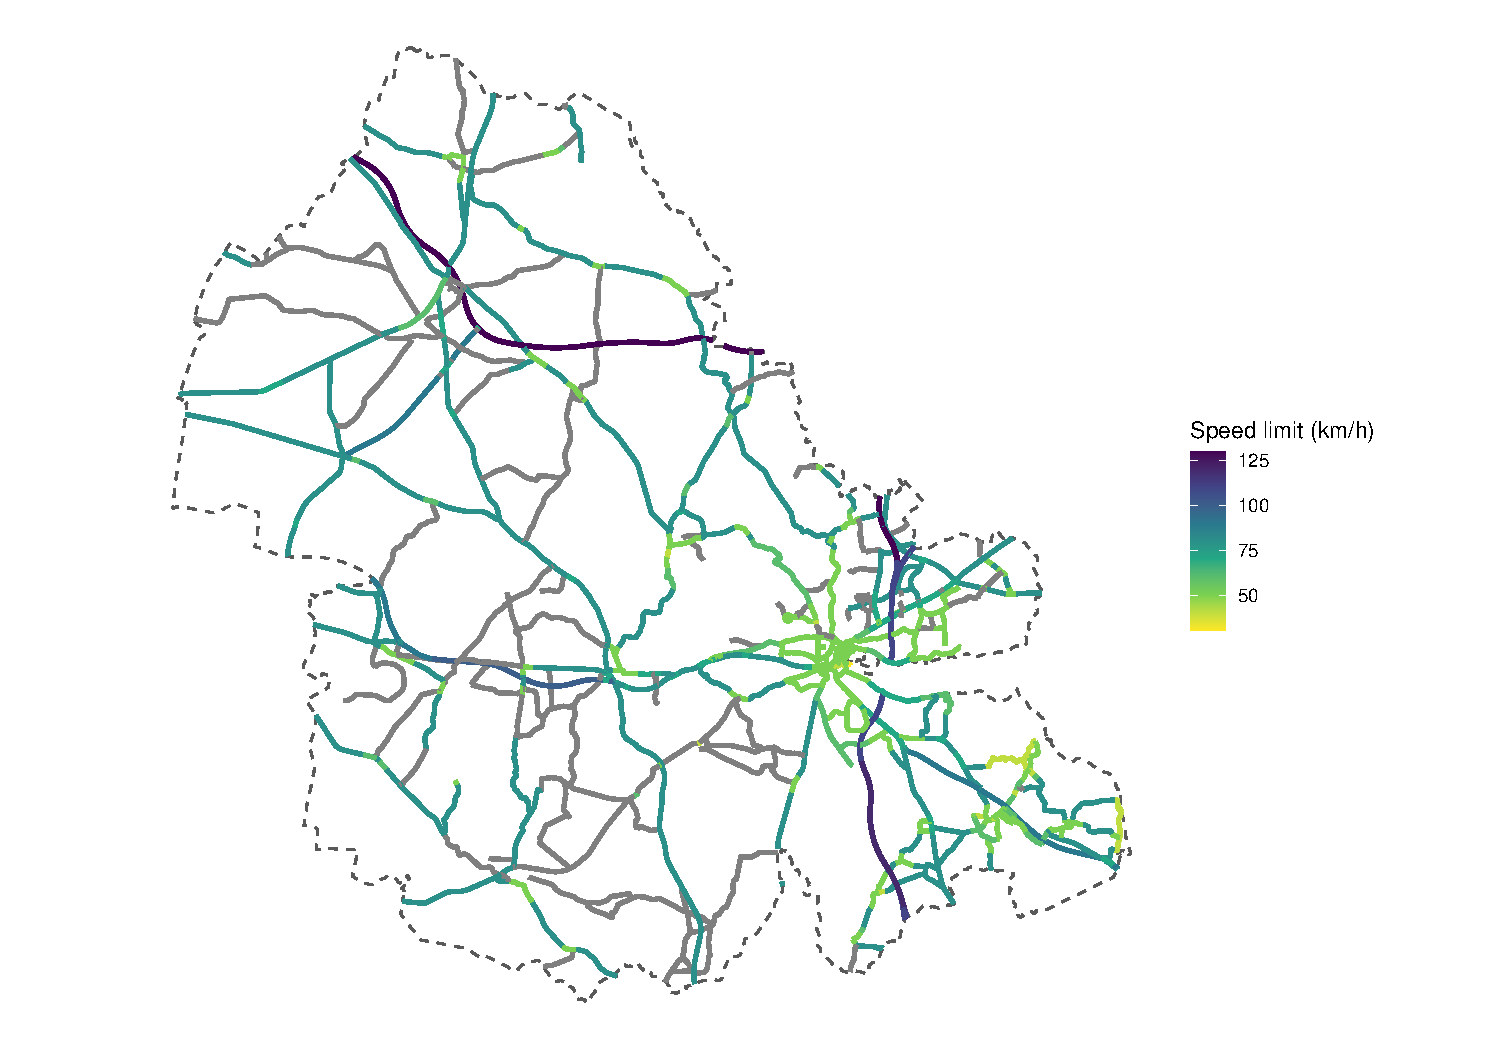
\includegraphics{crashcourse_slides_files/figure-beamer/unnamed-chunk-33-1.pdf}

\normalsize \columnsend
\end{frame}

\end{document}
